\documentclass[a4paper,12pt,titlepage]{scrartcl}
\usepackage[sc]{mathpazo} % Schrift - wie Funcky und in PDF zu Fonts beschrieben
\usepackage[T1]{fontenc}
\usepackage[utf8]{inputenc}
\usepackage[a-1b]{pdfx}
\usepackage[ngerman]{babel}
\usepackage[amssymb]{SIunits} 
\usepackage{graphicx} 
\usepackage{subfigure}                         
\usepackage{float}
\usepackage[iso,german]{isodate} %his package provides commands to switch between different date formats
\usepackage{hyperref}
\usepackage{mdwlist} %less space for lists
\usepackage{listings}
\lstset{
  literate={ö}{{\"o}}1
           {ä}{{\"a}}1
           {ü}{{\"u}}1
}

\usepackage{fancyhdr}
\renewcommand{\headrulewidth}{0.5pt}
\renewcommand{\footrulewidth}{0.5pt}
%Abstand zwischen Absätzen, Zeilenabstände
\voffset26pt 
\parskip6pt
%\parindent1cm  %Rückt erste Zeile eines neuen Absatzes ein
\usepackage{setspace}
\onehalfspacing

\begin{document}
\pagenumbering{roman}
\titlehead
{
    \small
    {
        Technische Universität Ilmenau\\
        Fakulät IA\\
        Fachgebiet Rechnerarchitektur\\

        Praktikum Rechnerarchitektur 2\\
        WS 2021/22}
}

\title {Versuchsprotokoll}
\subtitle{Versuche Befehlsausführung und Mikrocontroller}
\author{}
\date{\today\\*[60pt]}
\maketitle  %Erstellt das Titelblatt wie oben definiert

%Einstellungen zur Kopf- und Fußzeile
\pagestyle{fancy}
\fancyhead[R]{Praktikumsbericht: RA2}
\pagenumbering{arabic}
\newpage

\section*{Versuch B: Befehlsausführung}
Simulative Untersuchung der Ausführung von Maschinenbefehlen in unterschiedlichen Pipeline-Architekturen

\subsection*{Aufgabe 1}
Untersuche die vorbereitete Befehlsfolge mit den drei vorgegebenen Grundstrukturen Standard-Pipeline, Superskalar-in-Order und Superskalar-out-of-Order. Beobachte den Programmablauf und machen dich mit der Bedienung vertraut! Schauen vor dem Simulationsstart auch die Parametereinstellungen für Sprungvorhersage und Result Forwarding an (hier können auch Änderungen vorgenommen werden) und interpretiere das Verhalten während der Simulation.

Code A1b
\begin{lstlisting}[basicstyle=\tiny]
        addiu   $t1, $zero, 11
        addiu   $t2, $zero, 0
loop:   addu  $t2, $t2, $t1
        addiu   $t1, $t1, -1
        bnez    $t1, loop
\end{lstlisting}
Alle Strukturen mit Result-Forwarding und 2-Bit Vorhersage.

\textbf{Beobachtung}:
\begin{itemize*}
    \item Standard Pipeline
    \begin{itemize*}
        \item Takte: 43
        \item Befehle: 39
        \item Befehle pro Takt: 0,81
        \item Sprünge: 11
    \end{itemize*}
    \item Superskalar In-Order Pipeline (4 EX Einheiten)
    \begin{itemize*}
        \item Takte: 29
        \item Befehle: 44
        \item Befehle pro Takt: 1,21
        \item Sprünge: 11
    \end{itemize*}
    \item Superskalar Out-of-Order ( 4 EX Einheiten)
    \begin{itemize*}
        \item Takte: 20
        \item Befehle: 58
        \item Sprünge: 12
    \end{itemize*}
\end{itemize*}

\subsection*{Aufgabe 2}
Untersuche die Befehlsfolgen A4 und B2 mit mindestens je drei unterschiedlichen Simulationsläufen! Wähle die benutzten Pipelinestrukturen und Parametereinstellungen selbst aus. Vergleiche die Ergebnisse mit den Lösungen aus der Übung und suche Erklärungen für eventuelle Unterschiede!

Code A4
\begin{lstlisting}[basicstyle=\tiny]
lw      $t2, 4($t1)
addiu   $t3, $zero, 65
addu    $t5, $zero, $t2
sub     $t4, $t3, $t5
add     $t2, $t5, $t3
\end{lstlisting}

\textbf{Beobachtung}:
\begin{itemize*}
    \item Standard Pipeline
    \begin{itemize*}
        \item Takte: 11
        \item Befehle: 5
    \end{itemize*}
    \item Superskalar In-Order Pipeline (4 EX Einheiten)
    \begin{itemize*}
        \item Takte: 8
        \item Befehle: 5
        \item 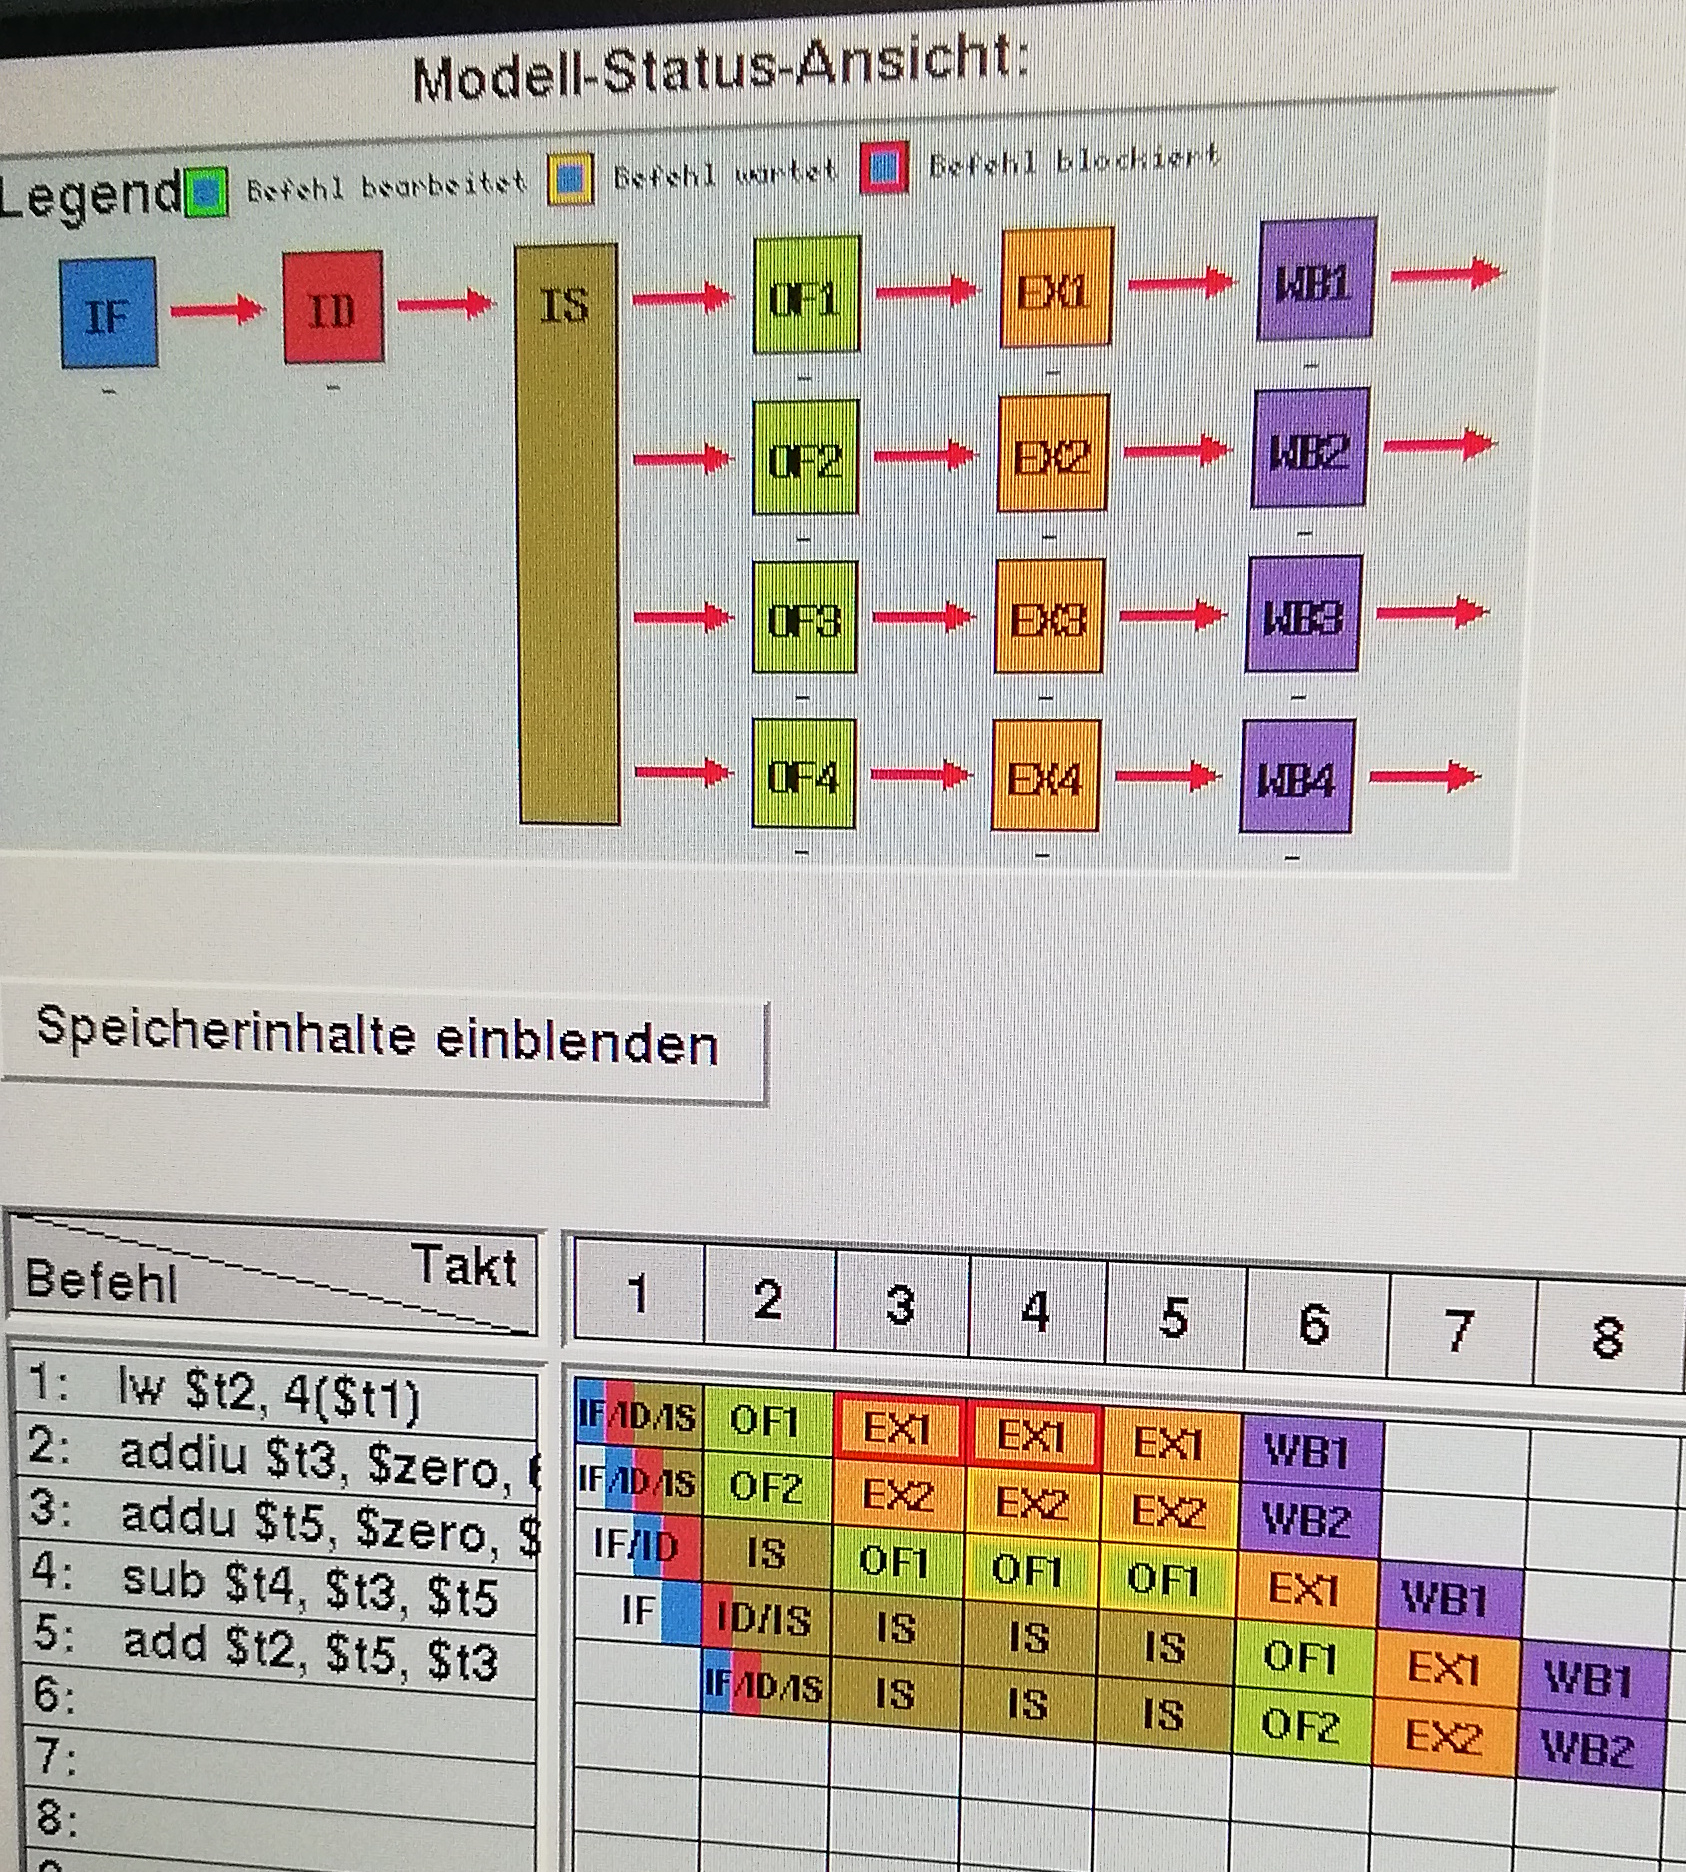
\includegraphics[width=.4\linewidth]{Assets/RA2-61330.jpg}
    \end{itemize*}
    \item Superskalar Out-of-Order ( 4 EX Einheiten)
    \begin{itemize*}
        \item Takte: 8
        \item Befehle: 5
    \end{itemize*}
\end{itemize*}

Code B2
\begin{lstlisting}[basicstyle=\tiny]
# addition der inhalte von 4 aufeinander folgenden speicherzellen, beginnend mit adresse 0x12345678 ...
# $t2 enthalte bereits den wert 0x12340000
    addi    $t0, $zero, 4           # max. zaehlerwert t0 = 4
    addi    $t2, $t2, 0x5678        # adressregister t2 = startadresse
    addi    $t3, $zero, 0           # zaehlerregister t3 = 0
    addi    $t1, $zero, 0           # ergebnisregister t1 = 0
loop:    lw      $t4, ($t2)         # tempregister t4 <- wert laden
    add     $t1, $t1, $t4           # summieren
    addi    $t2, $t2, 4             # adresse um 4 erhöhen
    addi    $t3, $t3, 1             # zaehler +1
    bne     $t3, $t0, loop          # loop für zaehler != 4
\end{lstlisting}

\textbf{Beobachtung}:
2 Bit Vorhersage
\begin{itemize*}
    \item Standard Pipeline
    \begin{itemize*}
        \item Takte: 40
        \item Befehle: 28
        \item 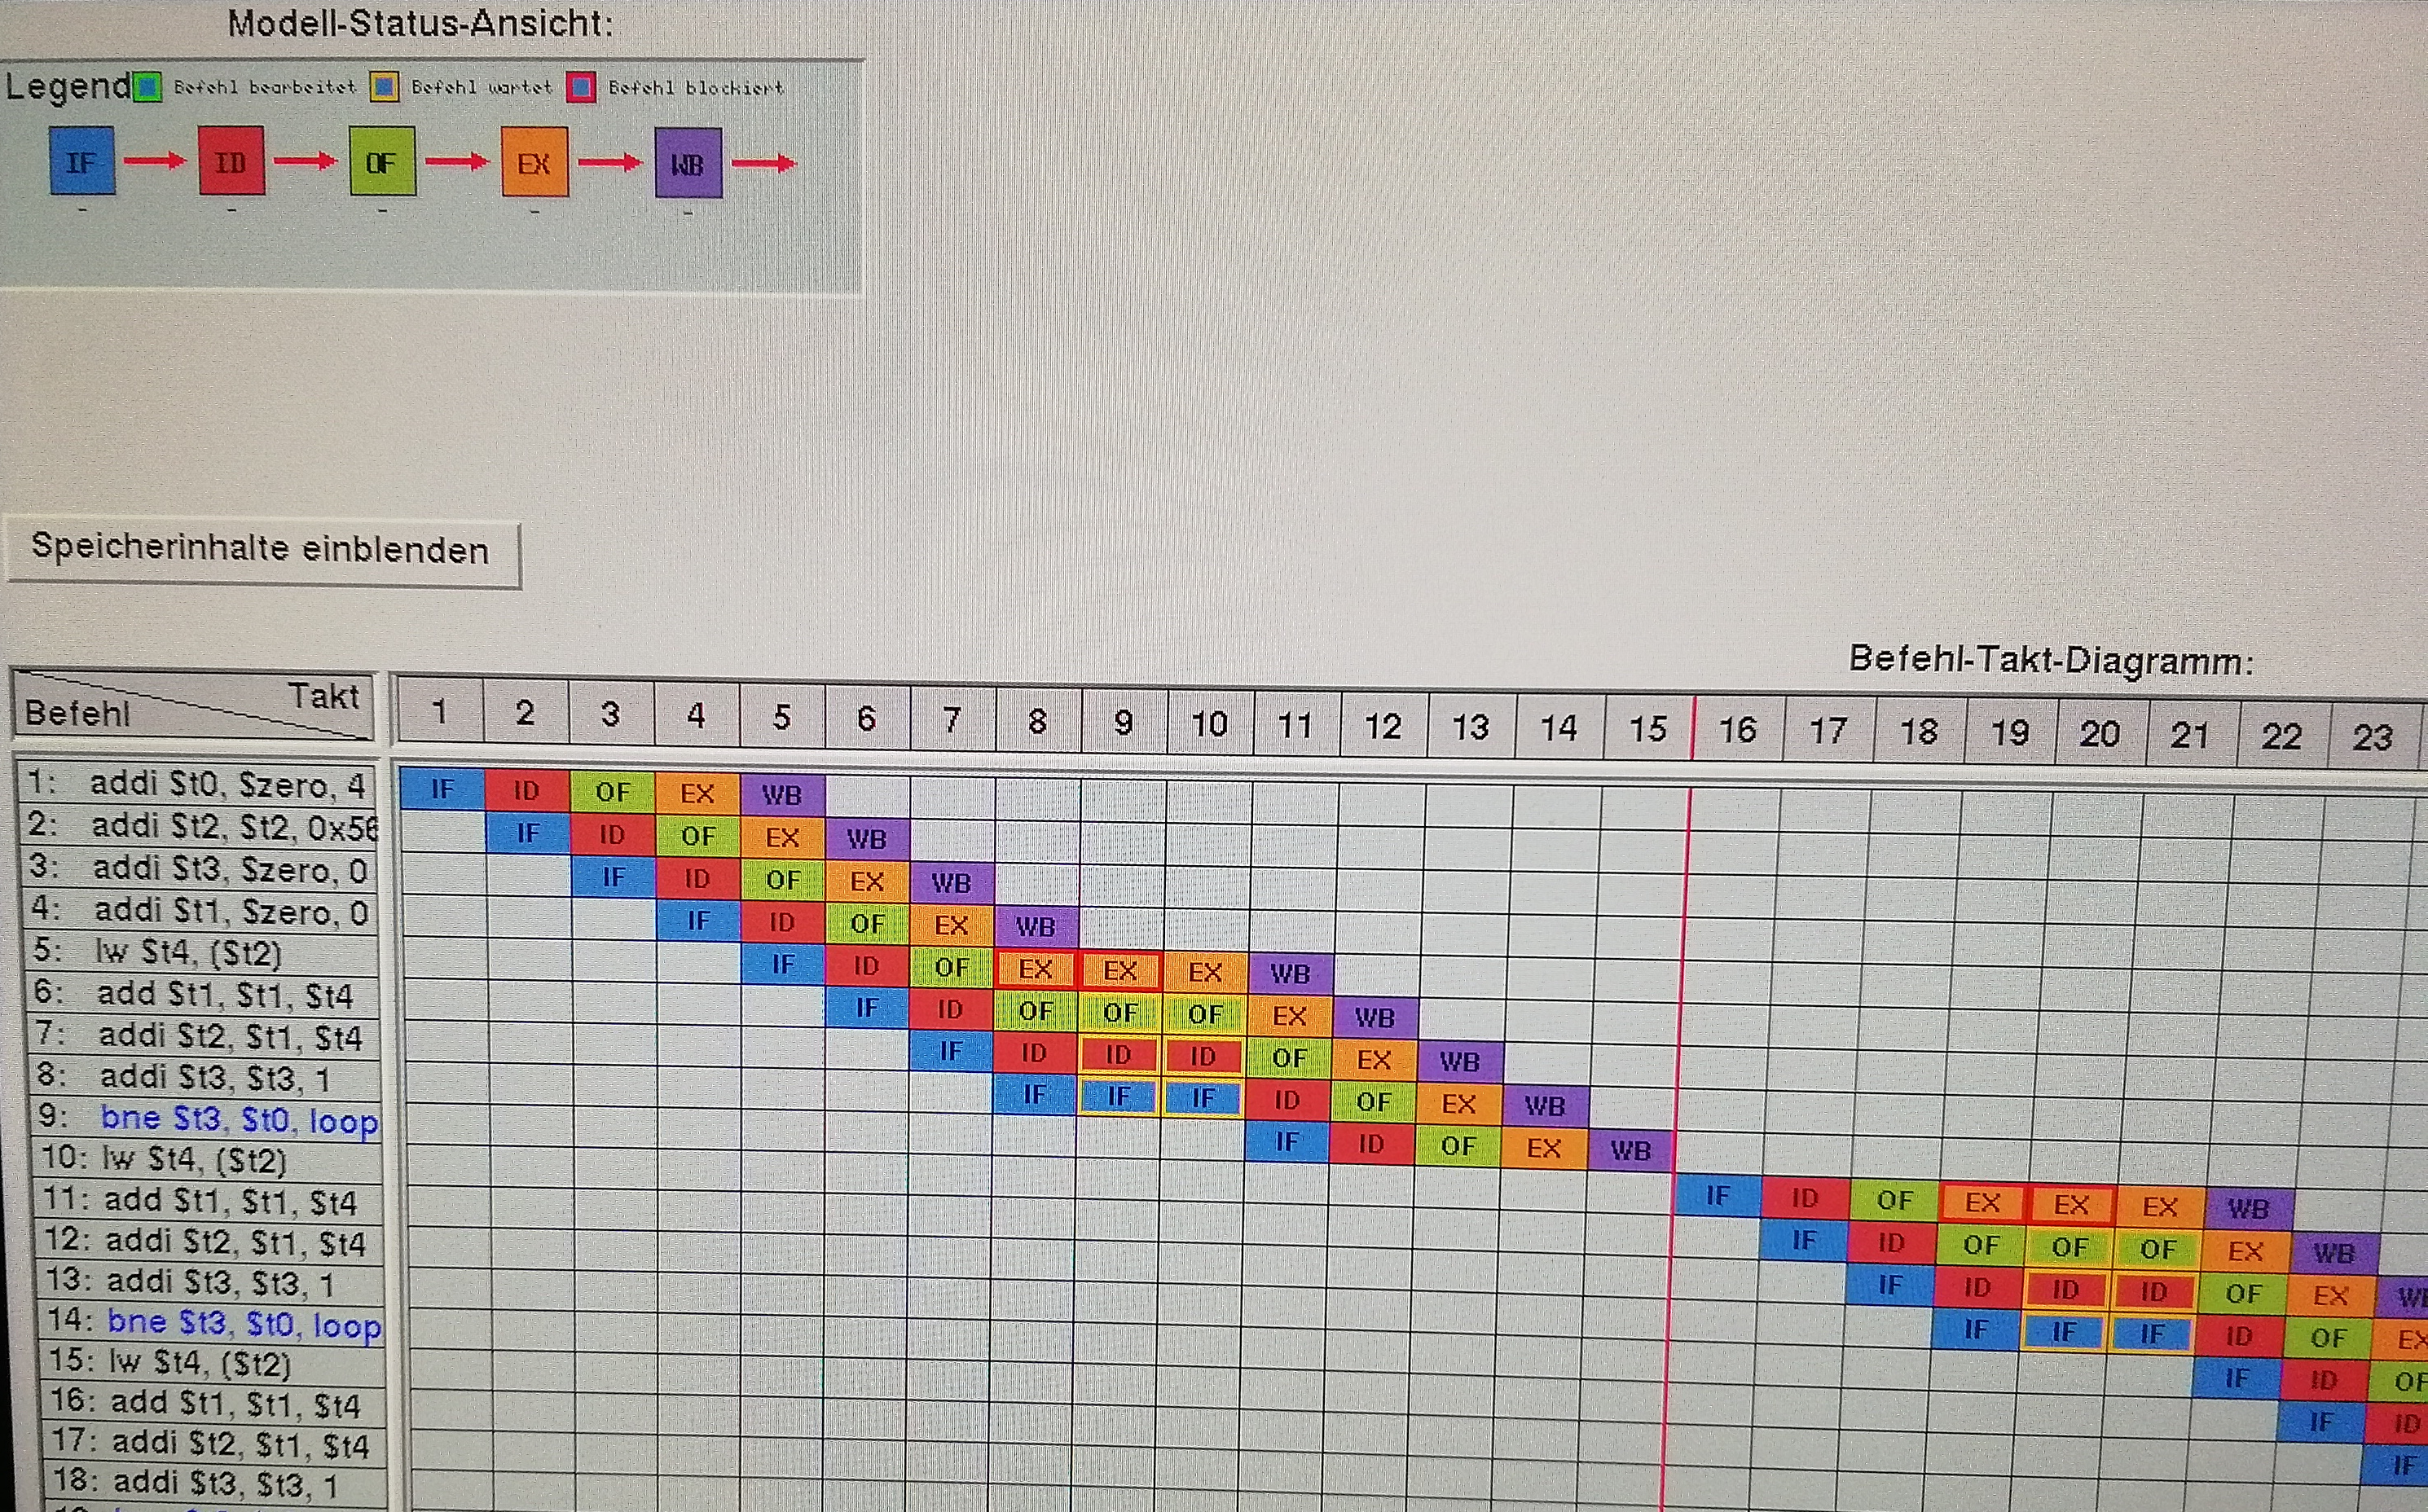
\includegraphics[width=.4\linewidth]{Assets/RA2-62418.jpg}
    \end{itemize*}
    \item Superskalar In-Order Pipeline (4 EX Einheiten)
    \begin{itemize*}
        \item Takte: 31
        \item Befehle: 32
        \item 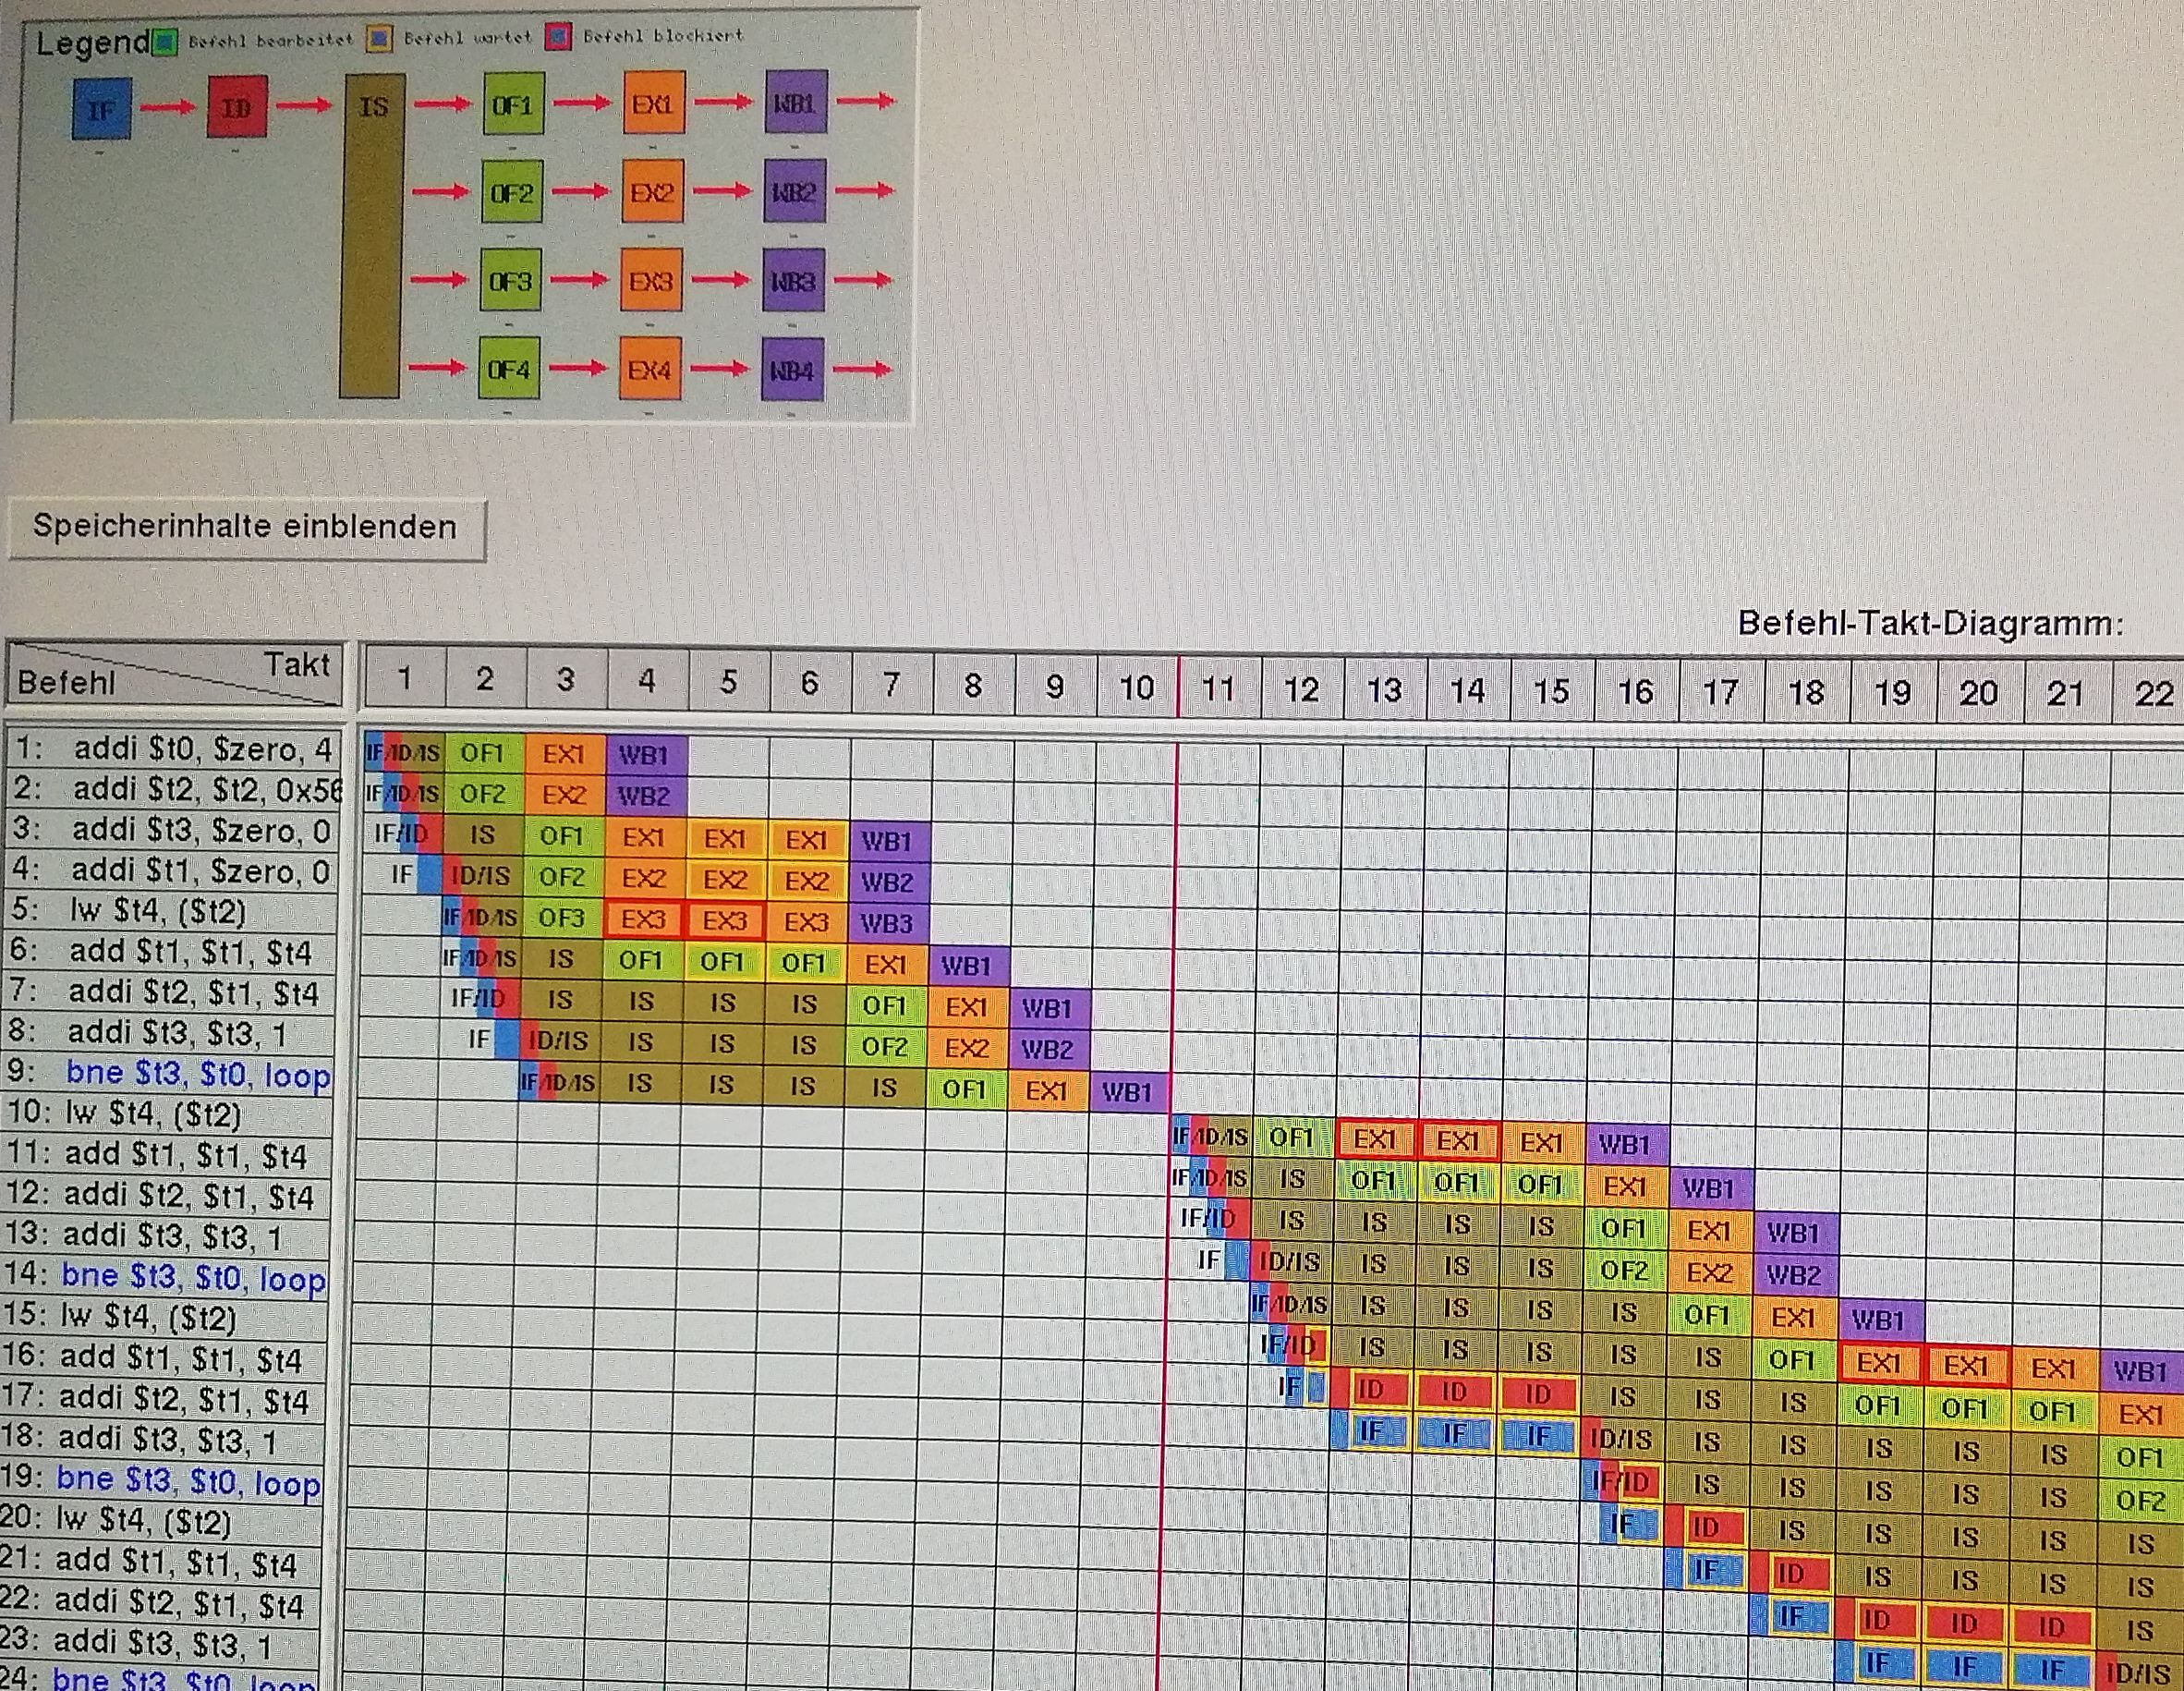
\includegraphics[width=.4\linewidth]{Assets/RA2-62729.jpg}
    \end{itemize*}
    \item Superskalar Out-of-Order ( 4 EX Einheiten)
    \begin{itemize*}
        \item Takte: 27
        \item Befehle: 80
        \item 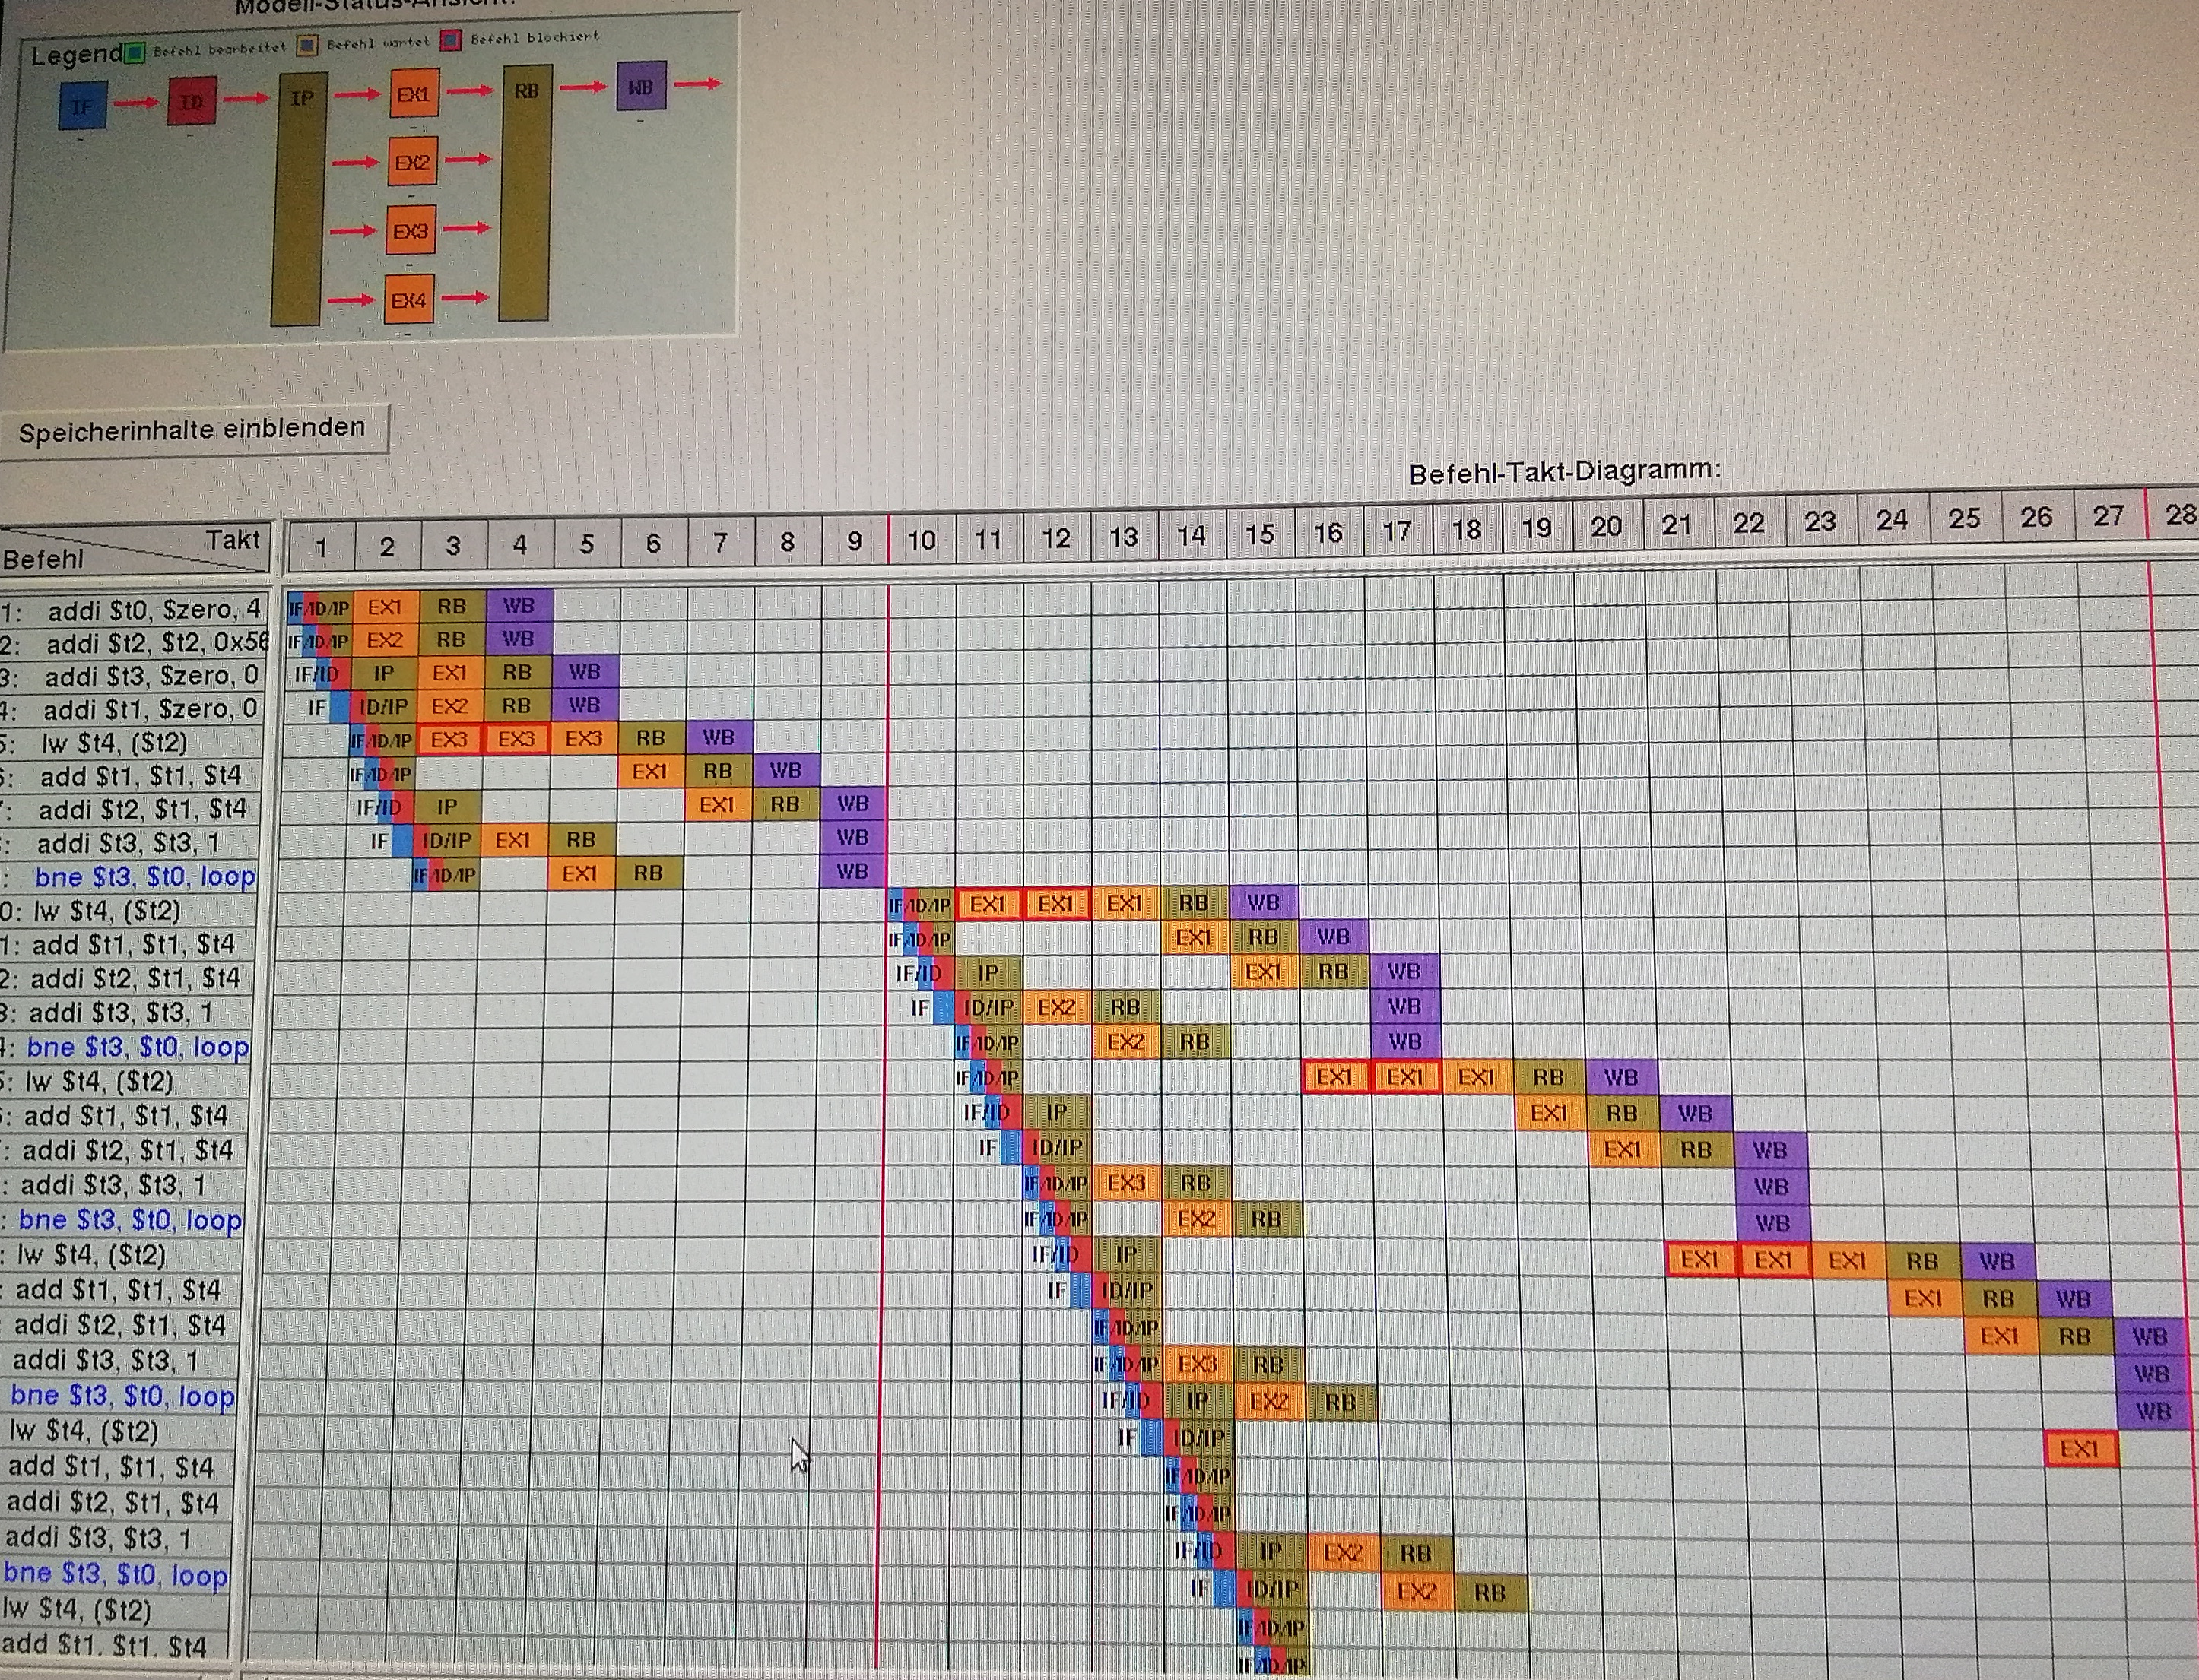
\includegraphics[width=.4\linewidth]{Assets/RA2-63122.jpg}
    \end{itemize*}
\end{itemize*}

1 Bit Vorhersage
\begin{itemize*}
    \item Standard Pipeline
    \begin{itemize*}
        \item Takte: 40
        \item Befehle: 28
    \end{itemize*}
    \item Superskalar In-Order Pipeline (4 EX Einheiten)
    \begin{itemize*}
        \item Takte: 31
        \item Befehle: 32
        \item 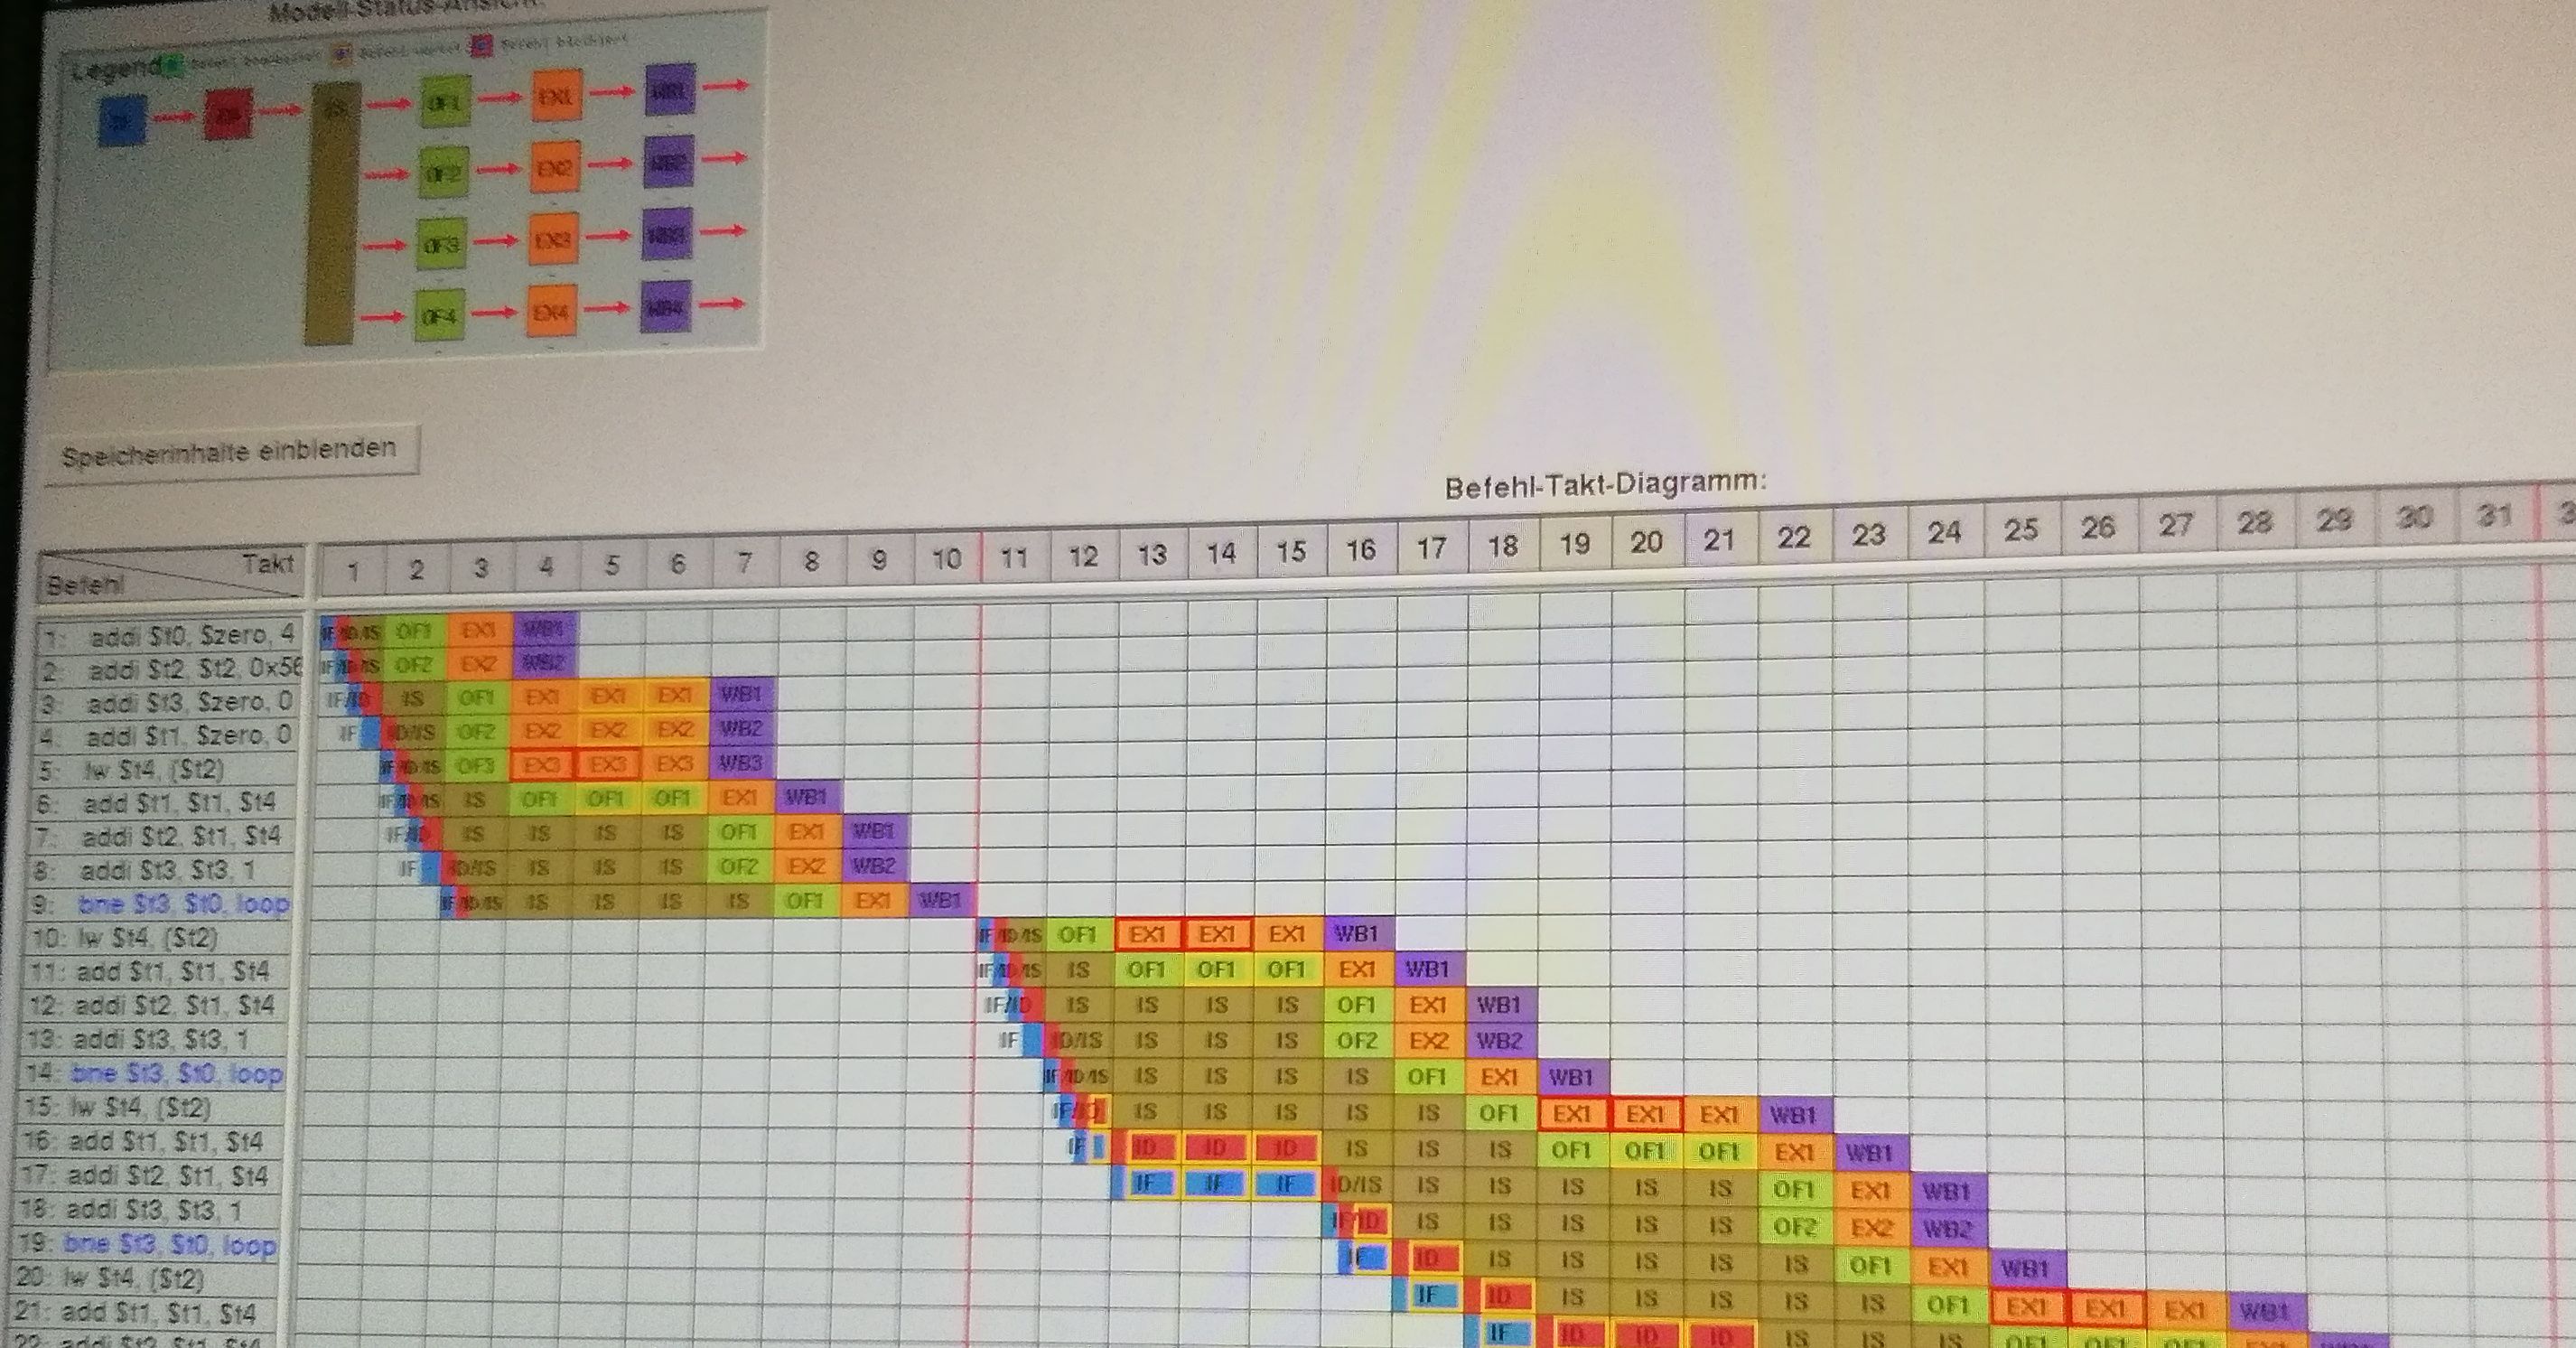
\includegraphics[width=.4\linewidth]{Assets/RA2-64222.jpg}
    \end{itemize*}
    \item Superskalar Out-of-Order ( 4 EX Einheiten)
    \begin{itemize*}
        \item Takte: 27
        \item Befehle: 80
        \item 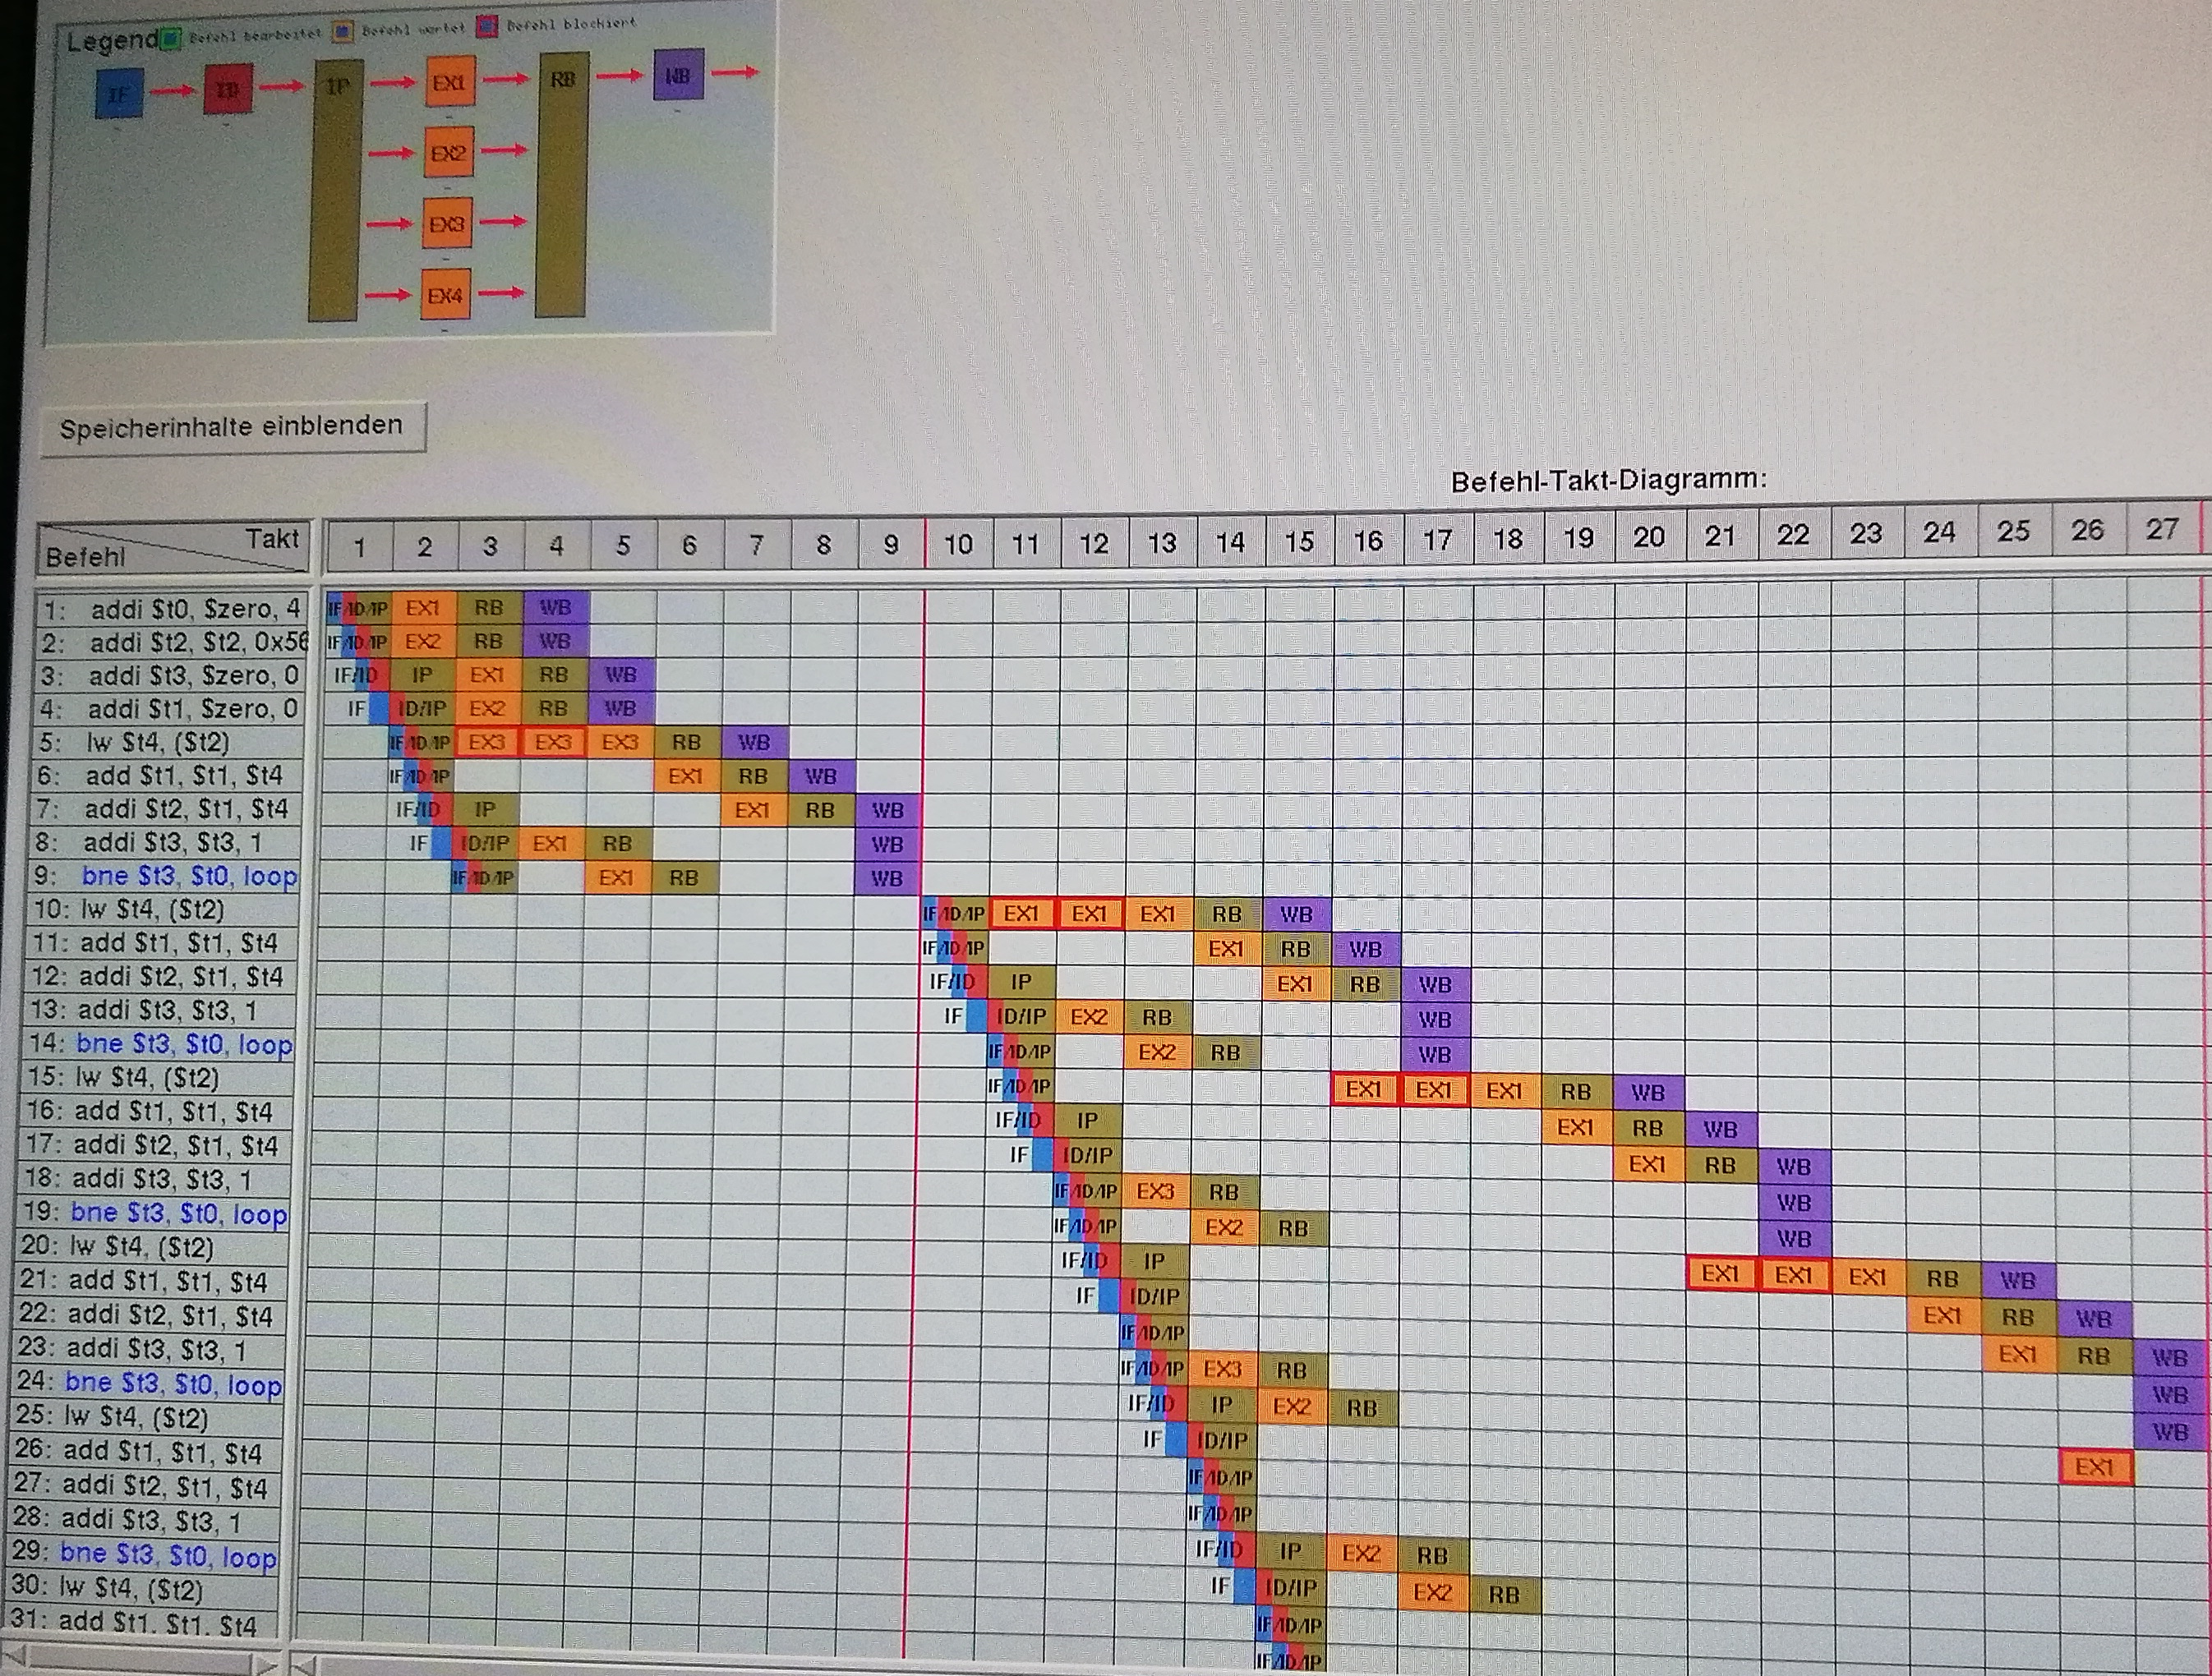
\includegraphics[width=.4\linewidth]{Assets/RA2-64400.jpg}
    \end{itemize*}
\end{itemize*}


0 Bit Vorhersage
\begin{itemize*}
    \item Standard Pipeline
    \begin{itemize*}
        \item Takte: 48
        \item Befehle: 24
        \item 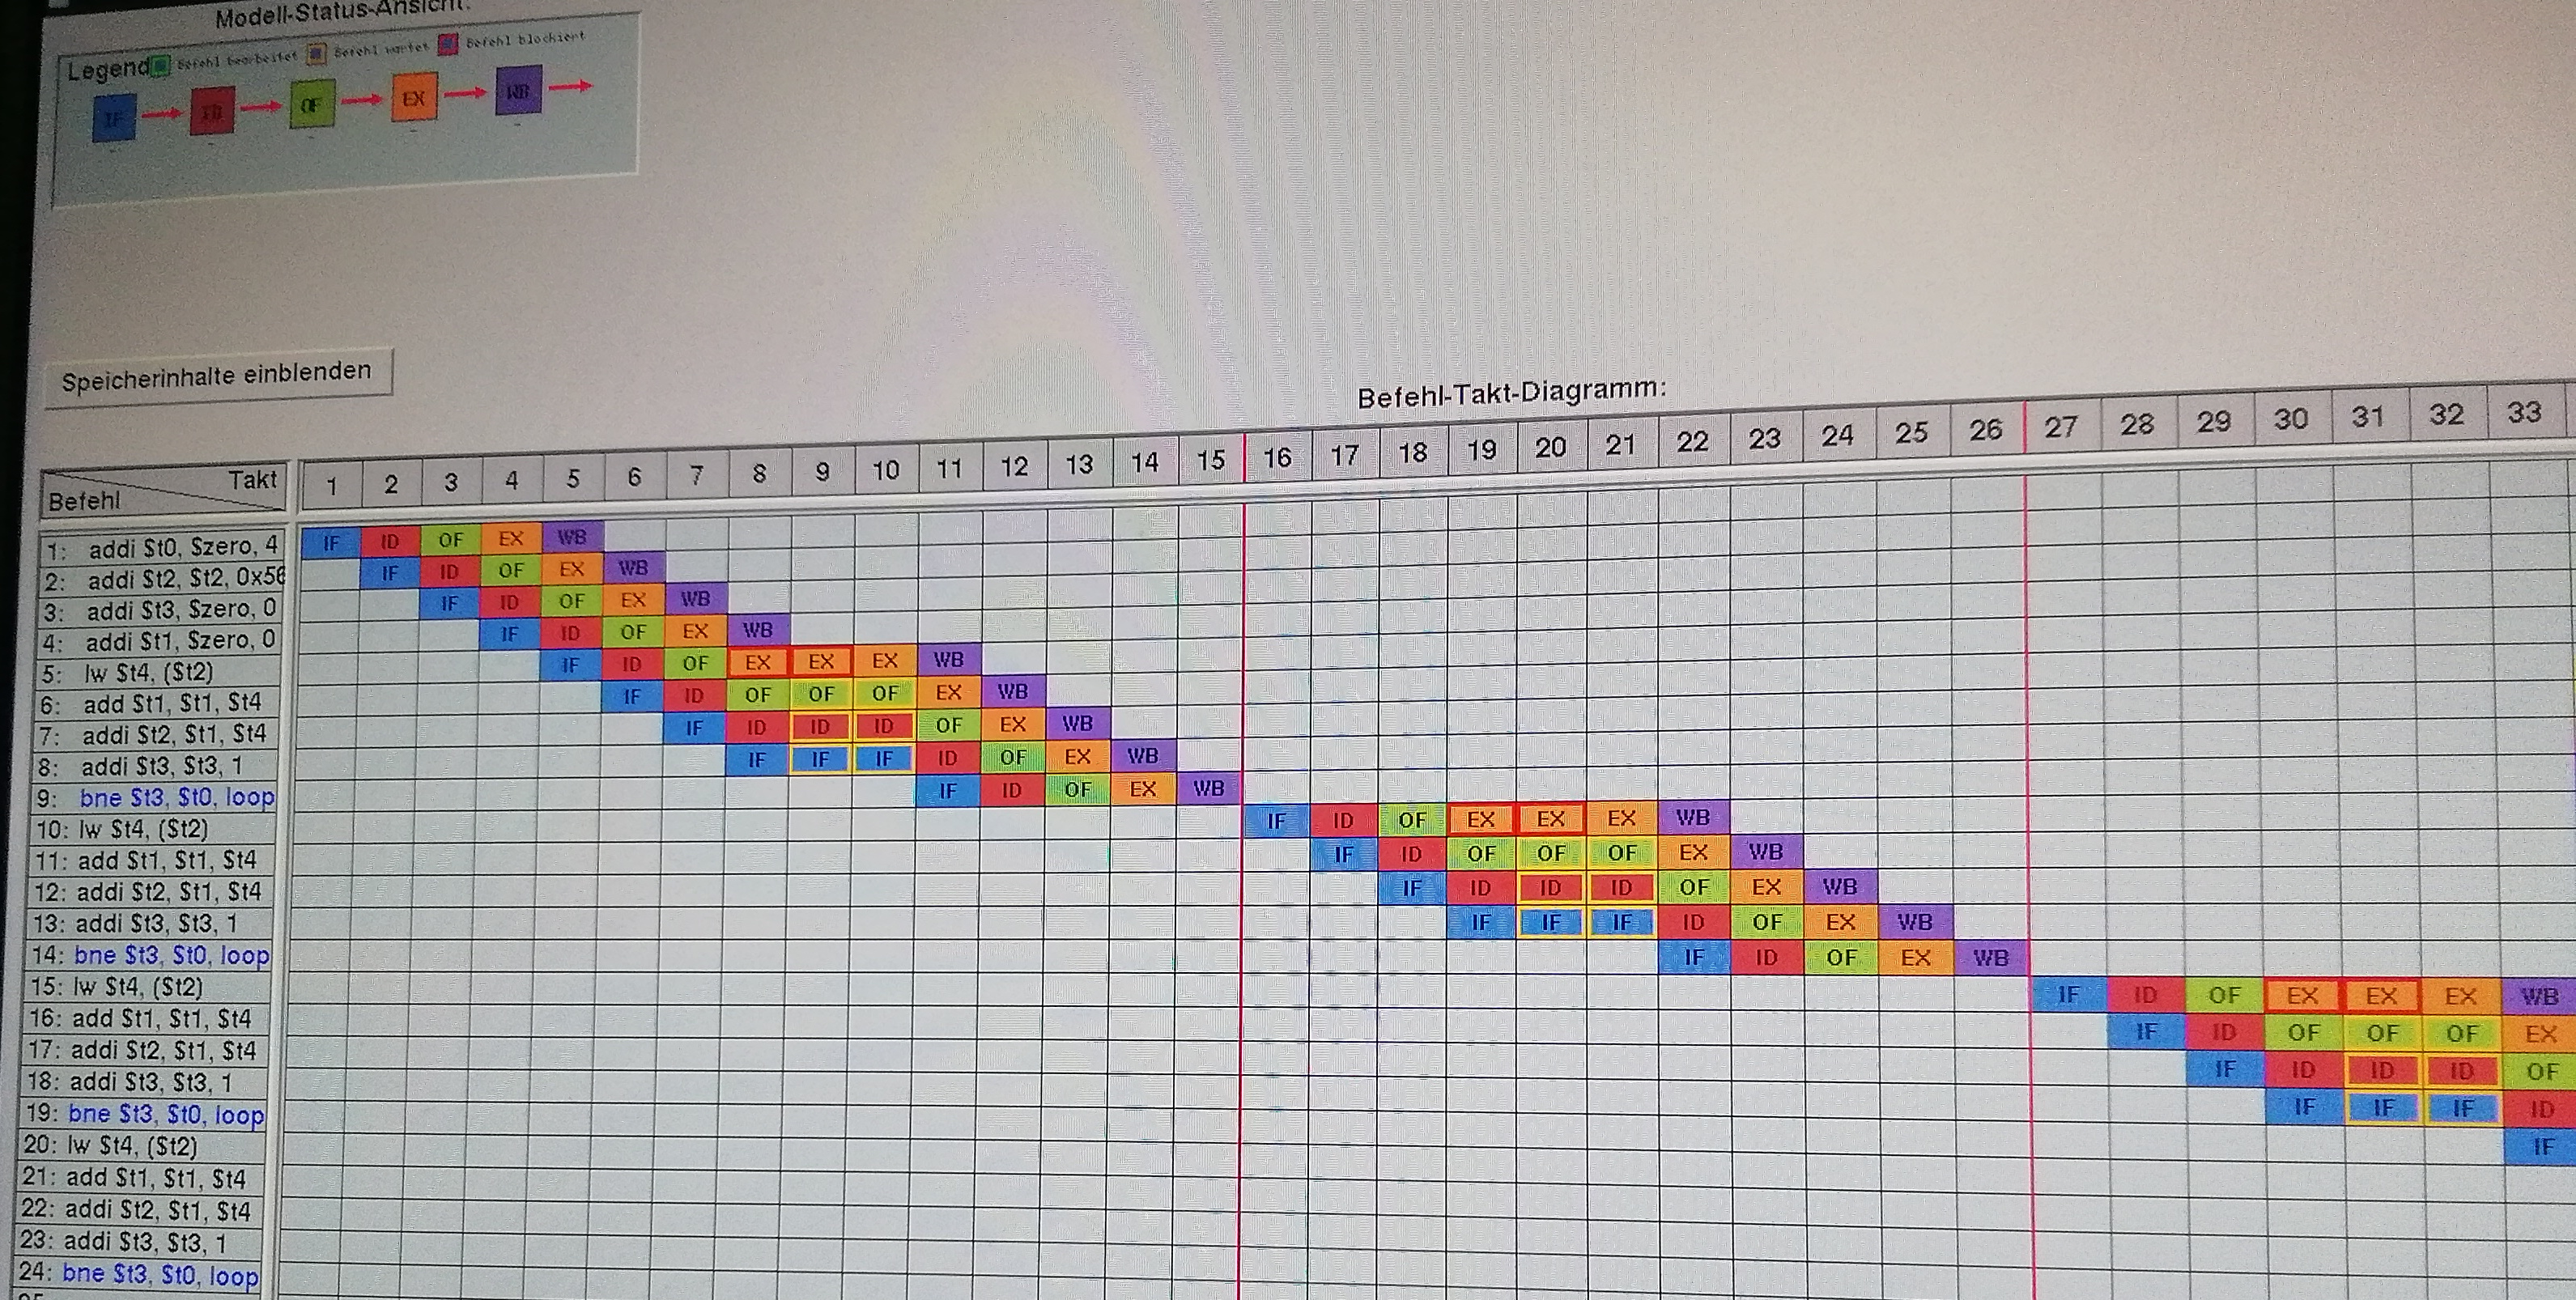
\includegraphics[width=.4\linewidth]{Assets/RA2-63915.jpg}
    \end{itemize*}
    \item Superskalar In-Order Pipeline (4 EX Einheiten)
    \begin{itemize*}
        \item Takte: 37
        \item Befehle: 24
        \item 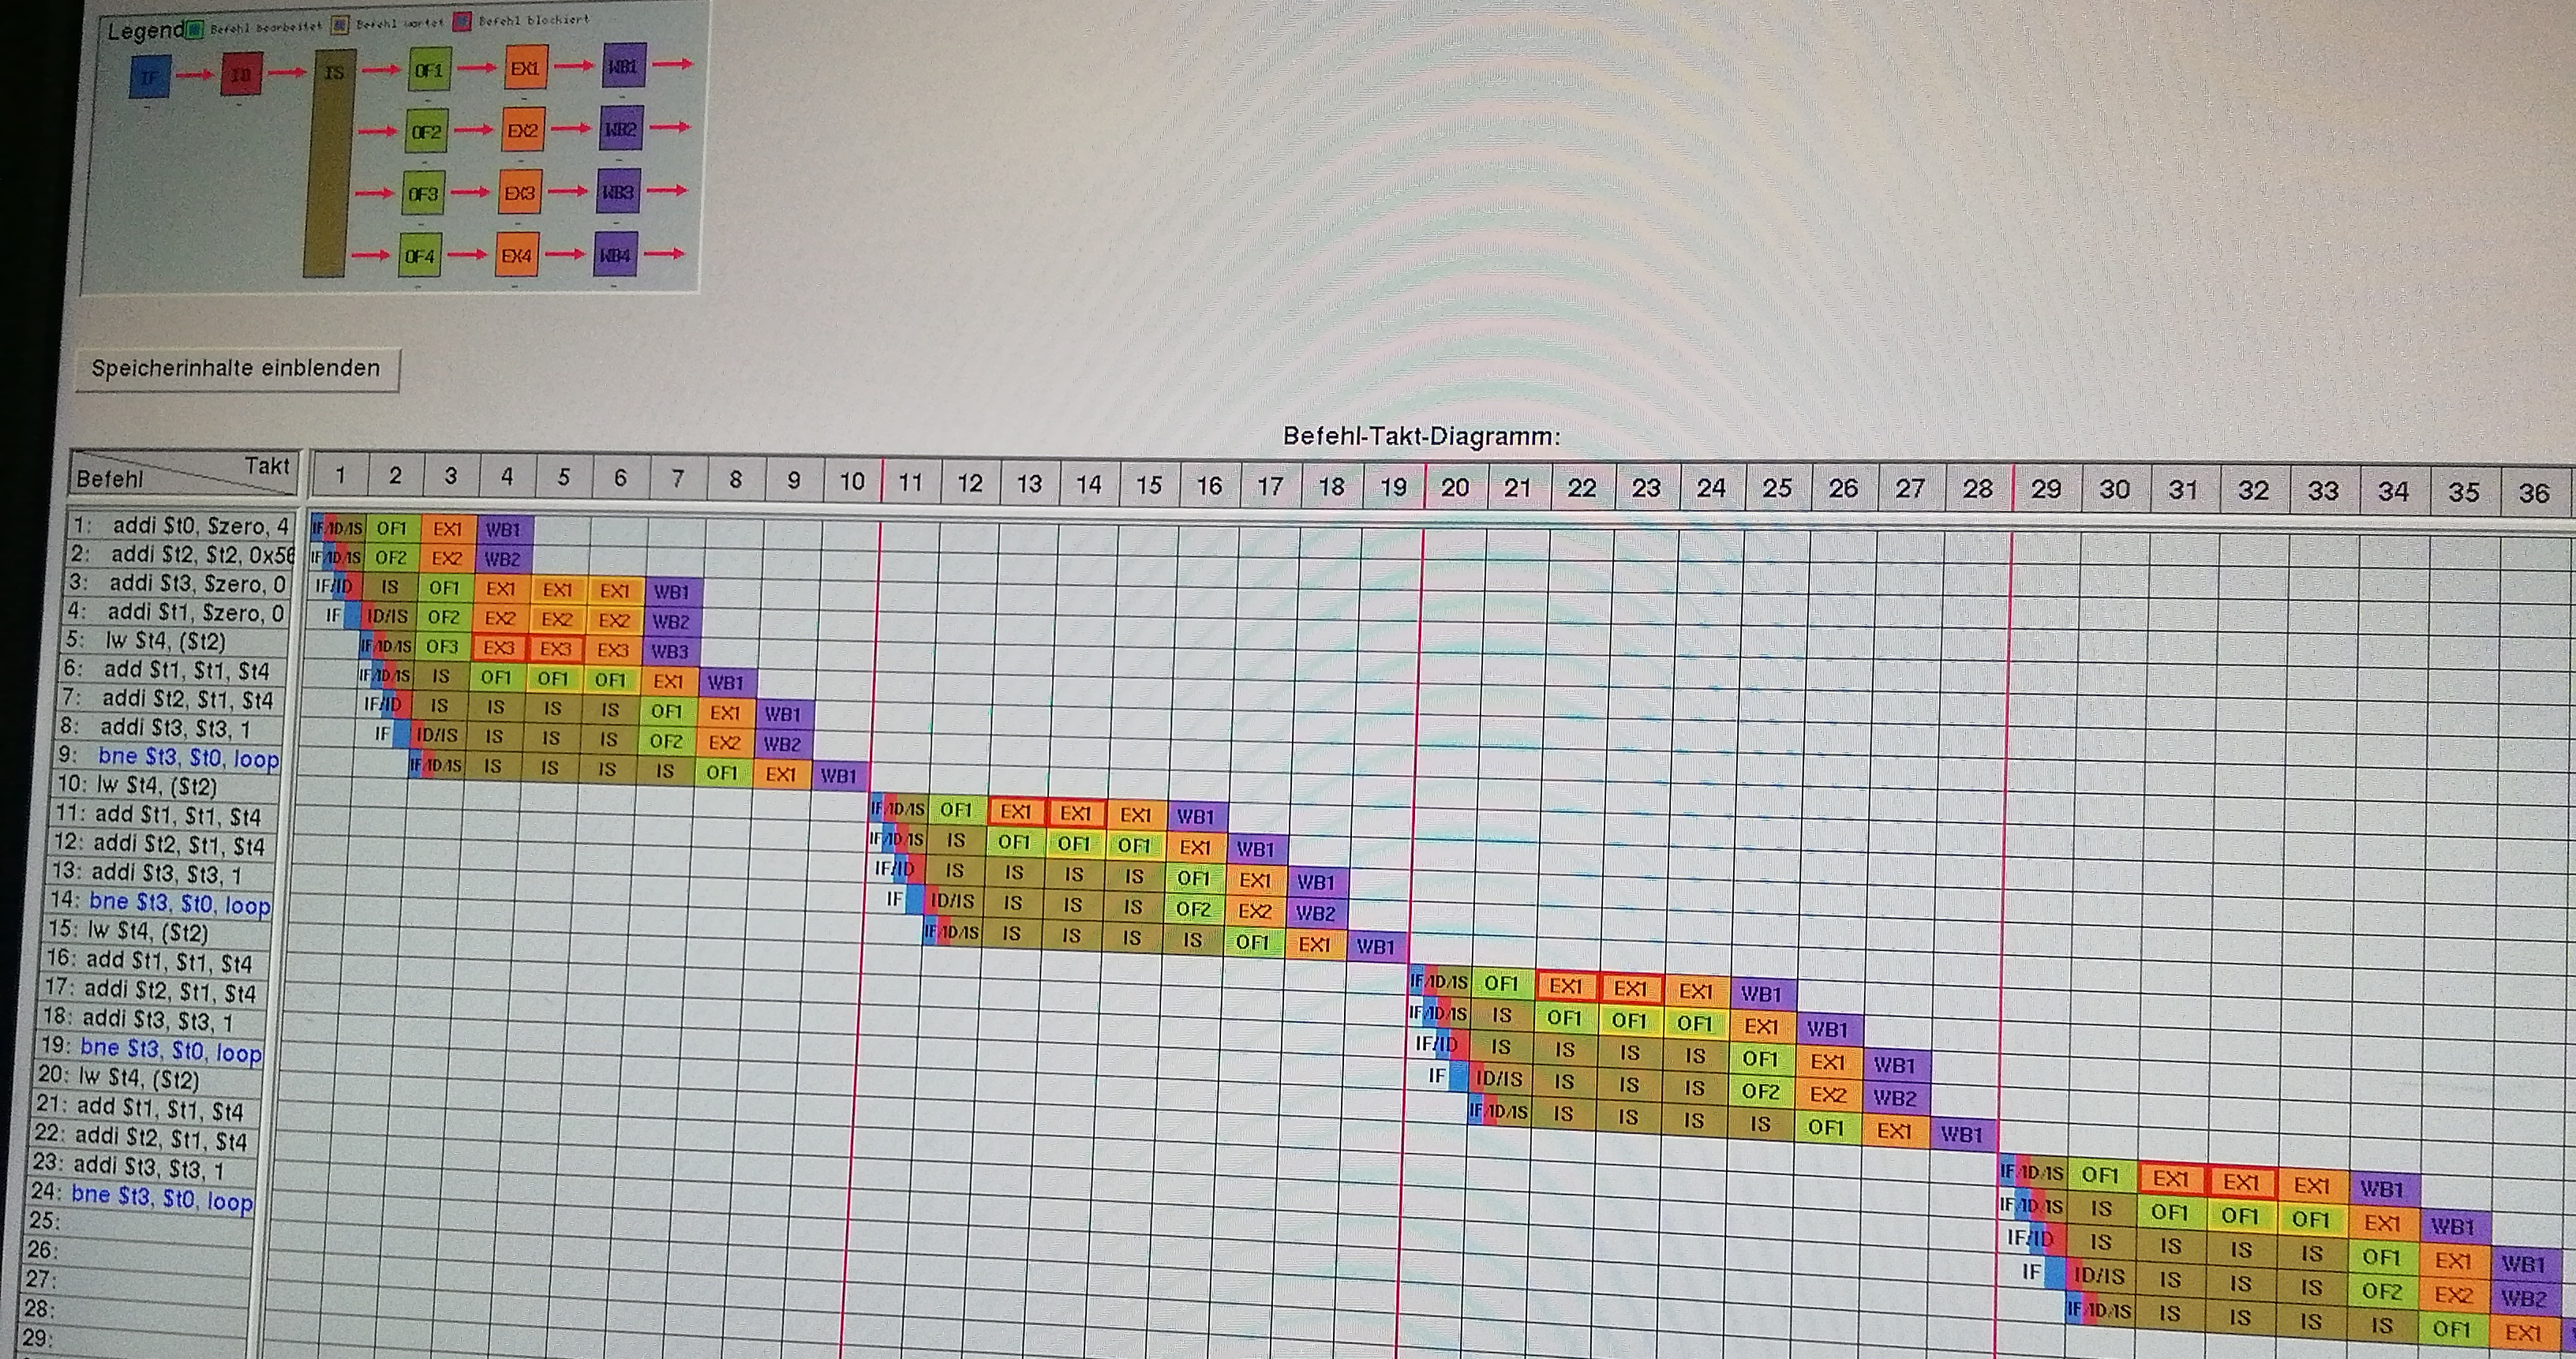
\includegraphics[width=.4\linewidth]{Assets/RA2-63642.jpg}
    \end{itemize*}
    \item Superskalar Out-of-Order ( 4 EX Einheiten)
    \begin{itemize*}
        \item Takte: 33
        \item Befehle: 24
        \item 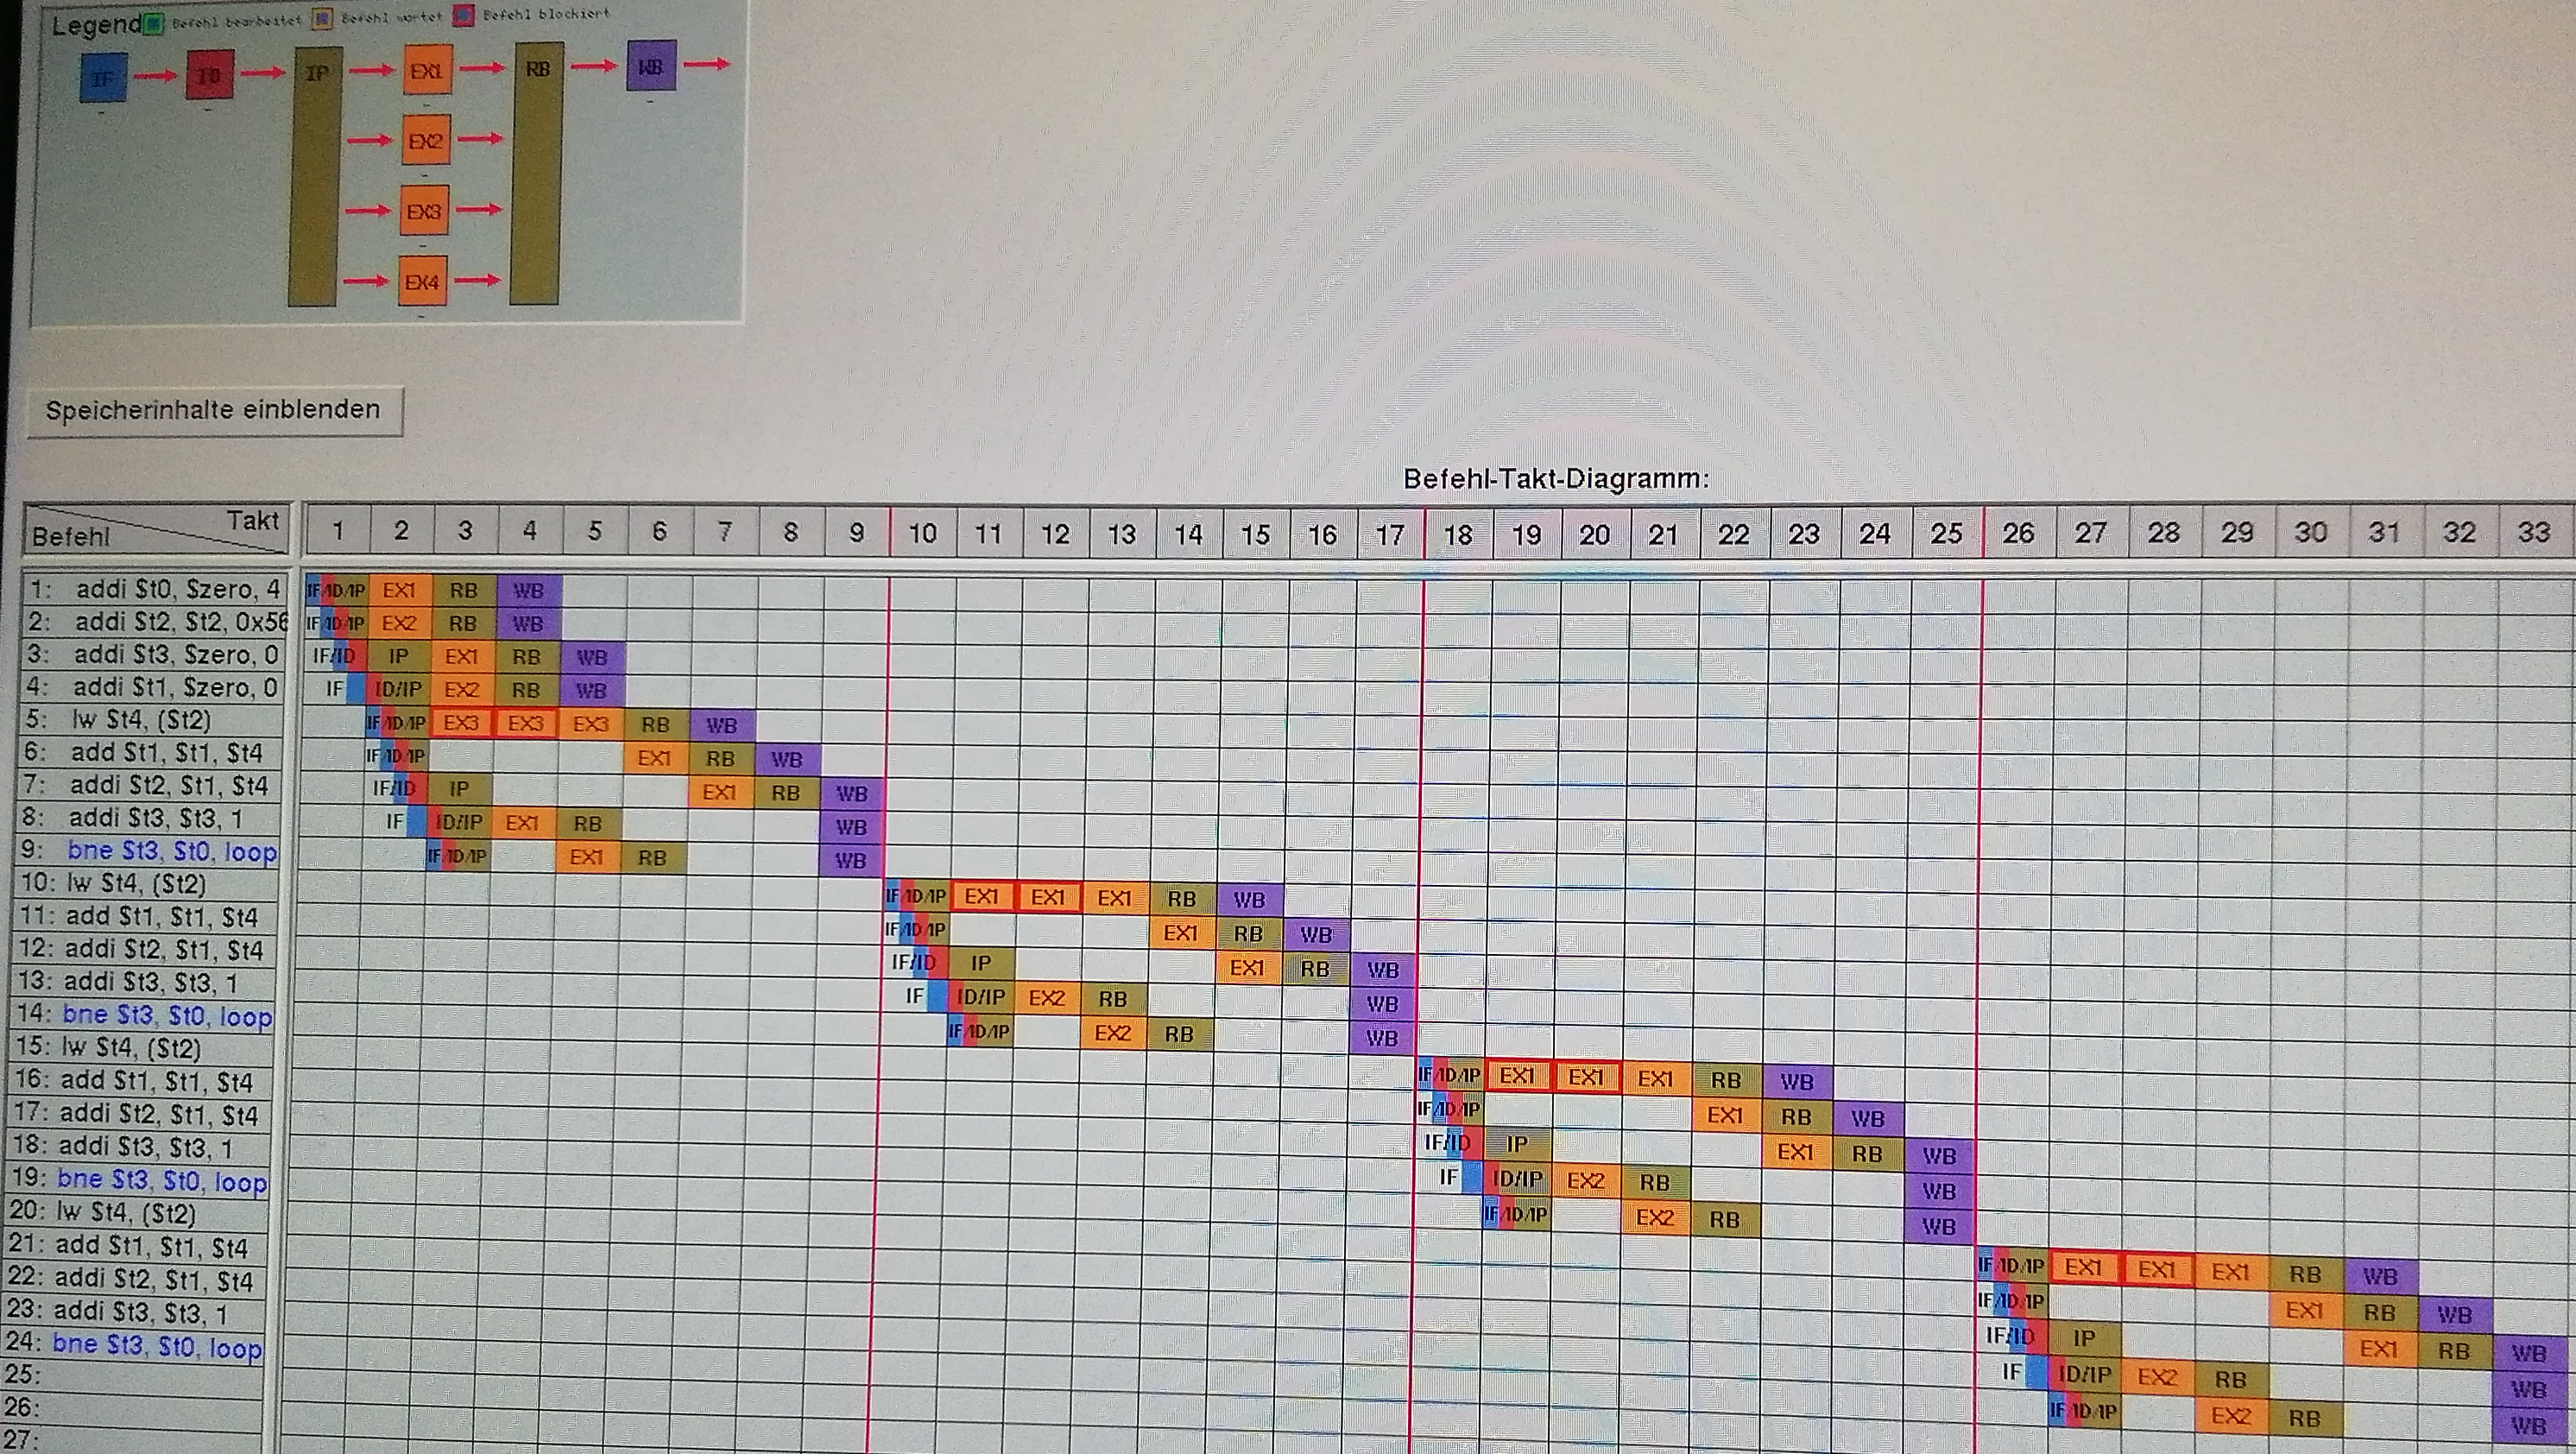
\includegraphics[width=.4\linewidth]{Assets/RA2-63323.jpg}
    \end{itemize*}
\end{itemize*}


Superskalar In-Order Pipeline ohne Result Forwarding (4 EX Einheiten)
\begin{itemize*}
    \item Takte: 57
    \item Befehle: 32
    \item 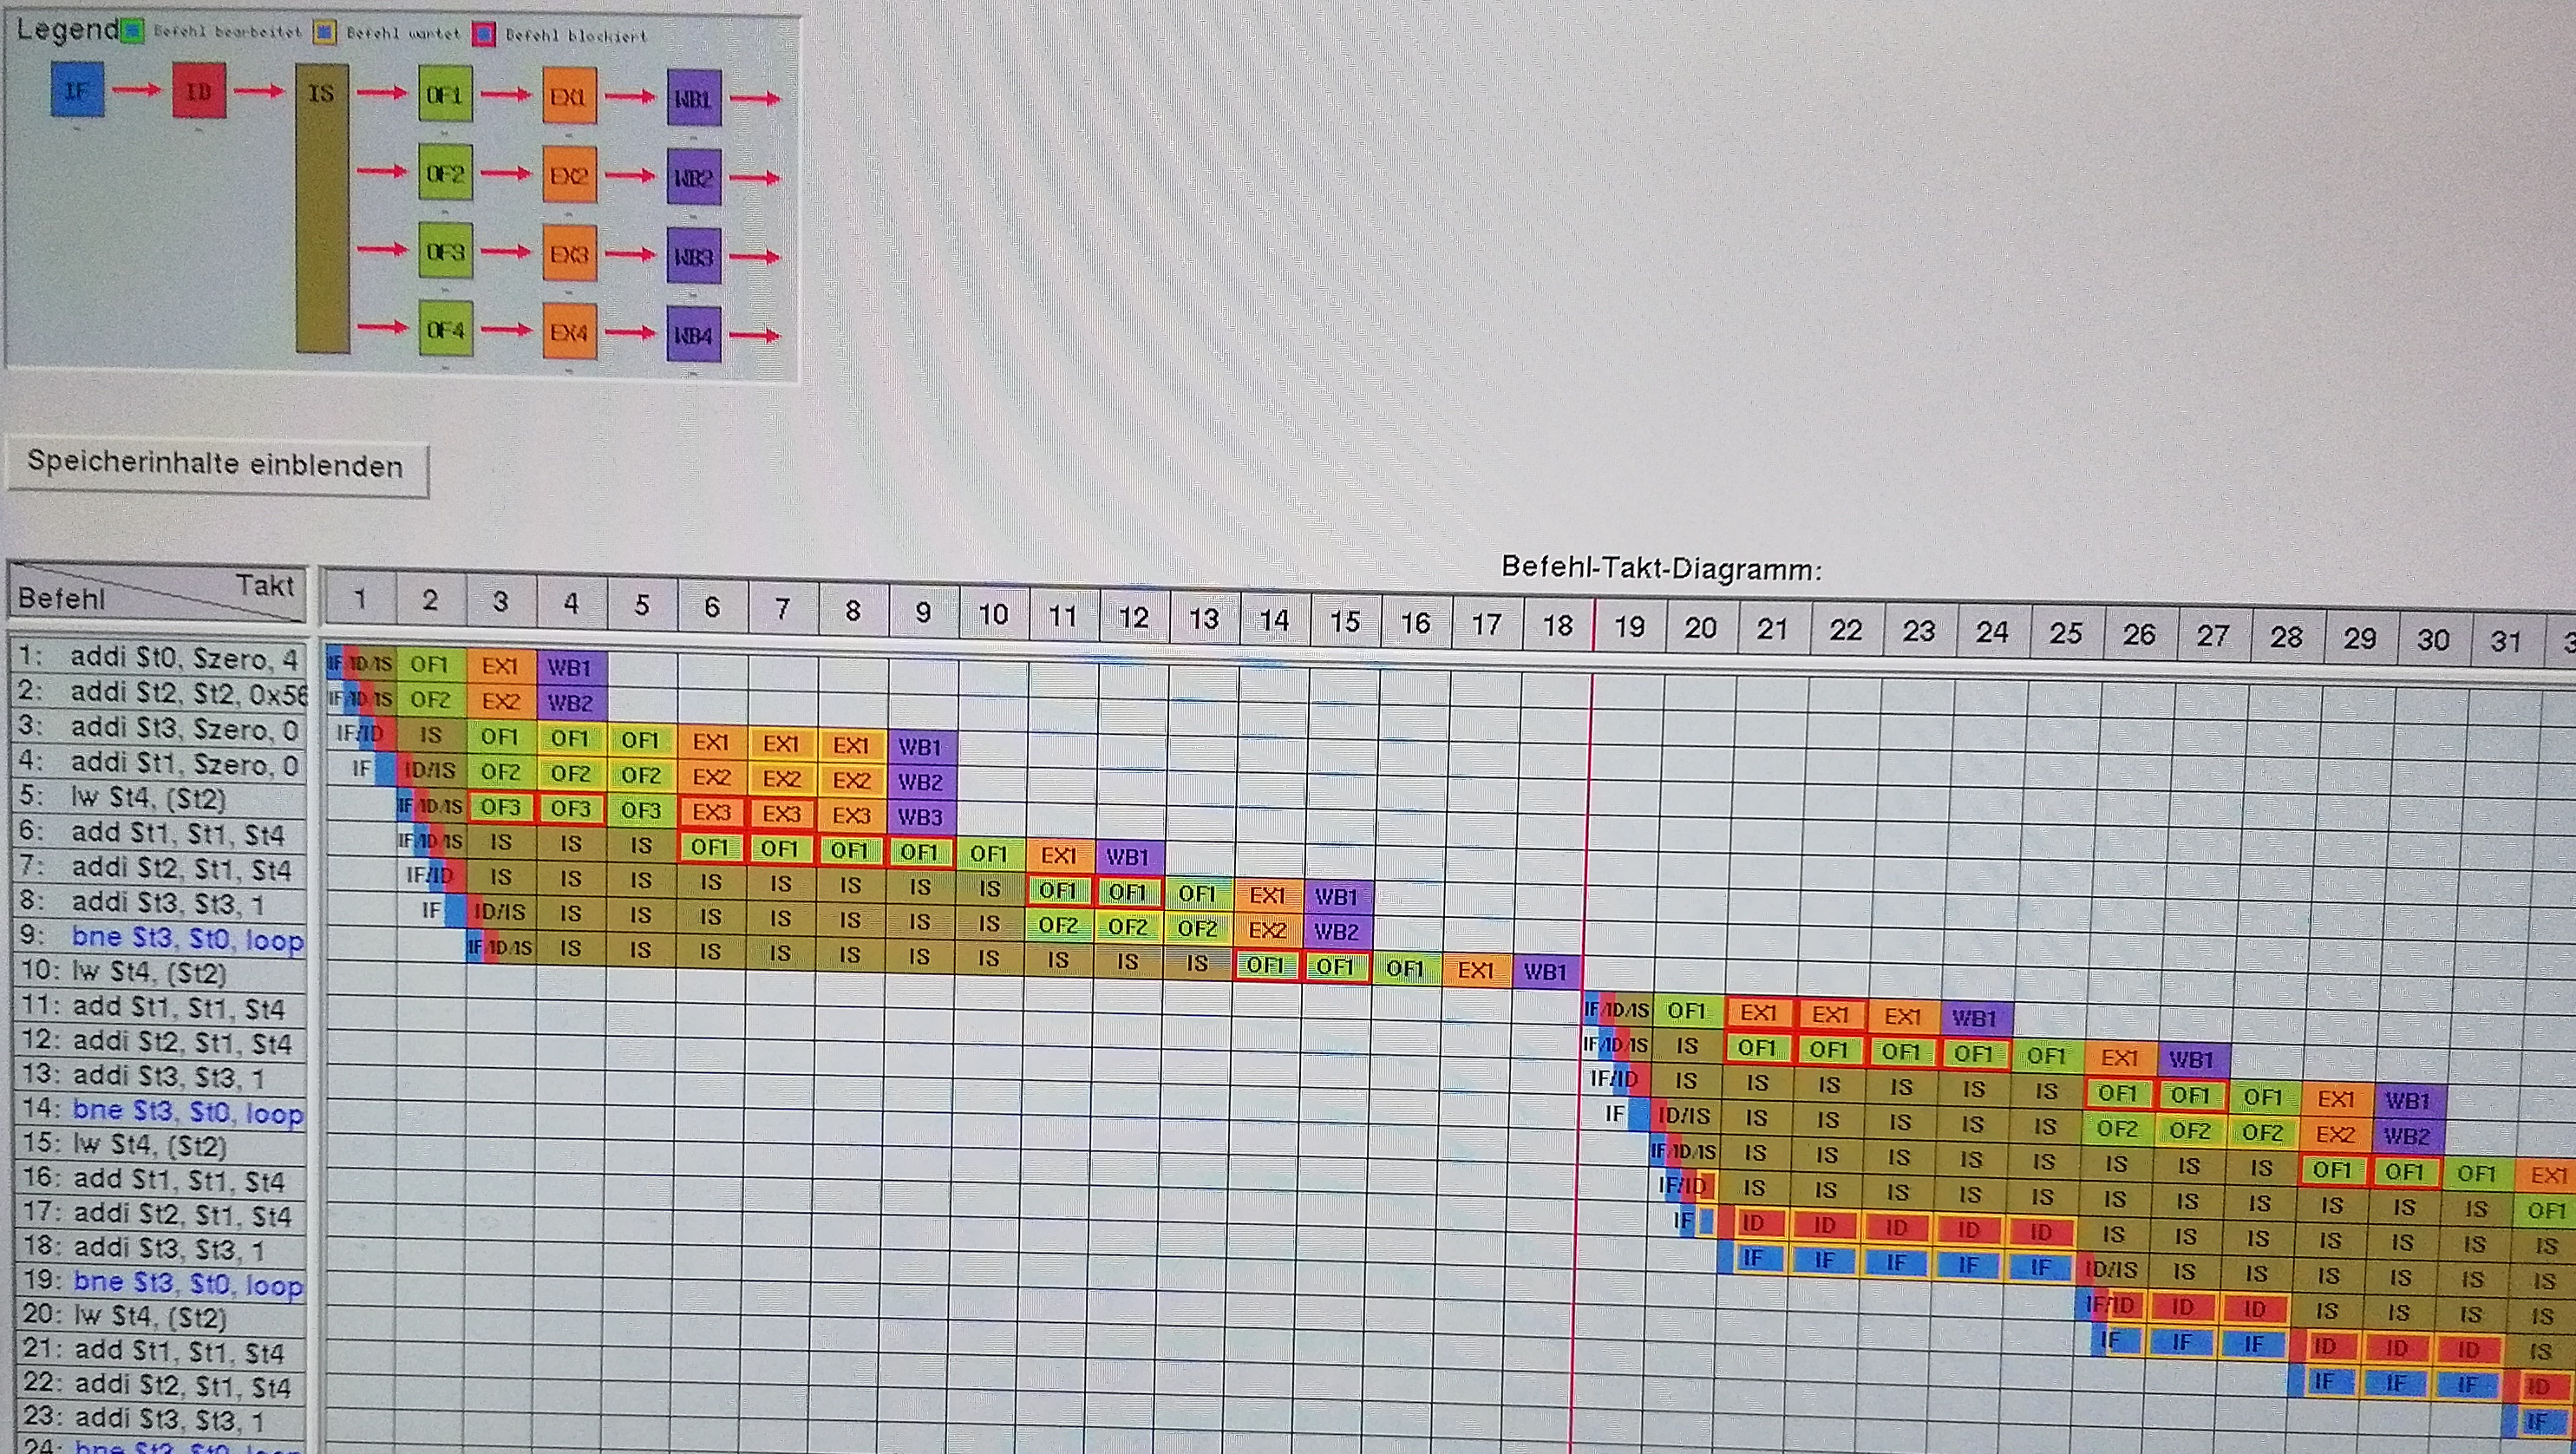
\includegraphics[width=.4\linewidth]{Assets/RA2-73350.jpg}
\end{itemize*}


\subsection*{Aufgabe 3}
Änderne nun eine der vorgegebenen Pipelinestrukturen ab, z.B. die Anzahl der parallelen Pipelines verändern. Orientiere dich zuvor über den Inhalt des ,,Baukastens''. Untersuche mit den oben verwendeten Befehlsfolgen die Auswirkungen auf die Simulationsergebnisse! Variiere dabei die Parameter und interpretiere die Ergebnisse!

\textbf{Beobachtung}: jeweils mit 2 Bit Vorhersage und Result Forwarding
\begin{itemize*}
    \item Superskalar In-Order Pipeline (3 EX Einheiten)
    \begin{itemize*}
        \item Takte: 32
        \item Befehle: 31
        \item 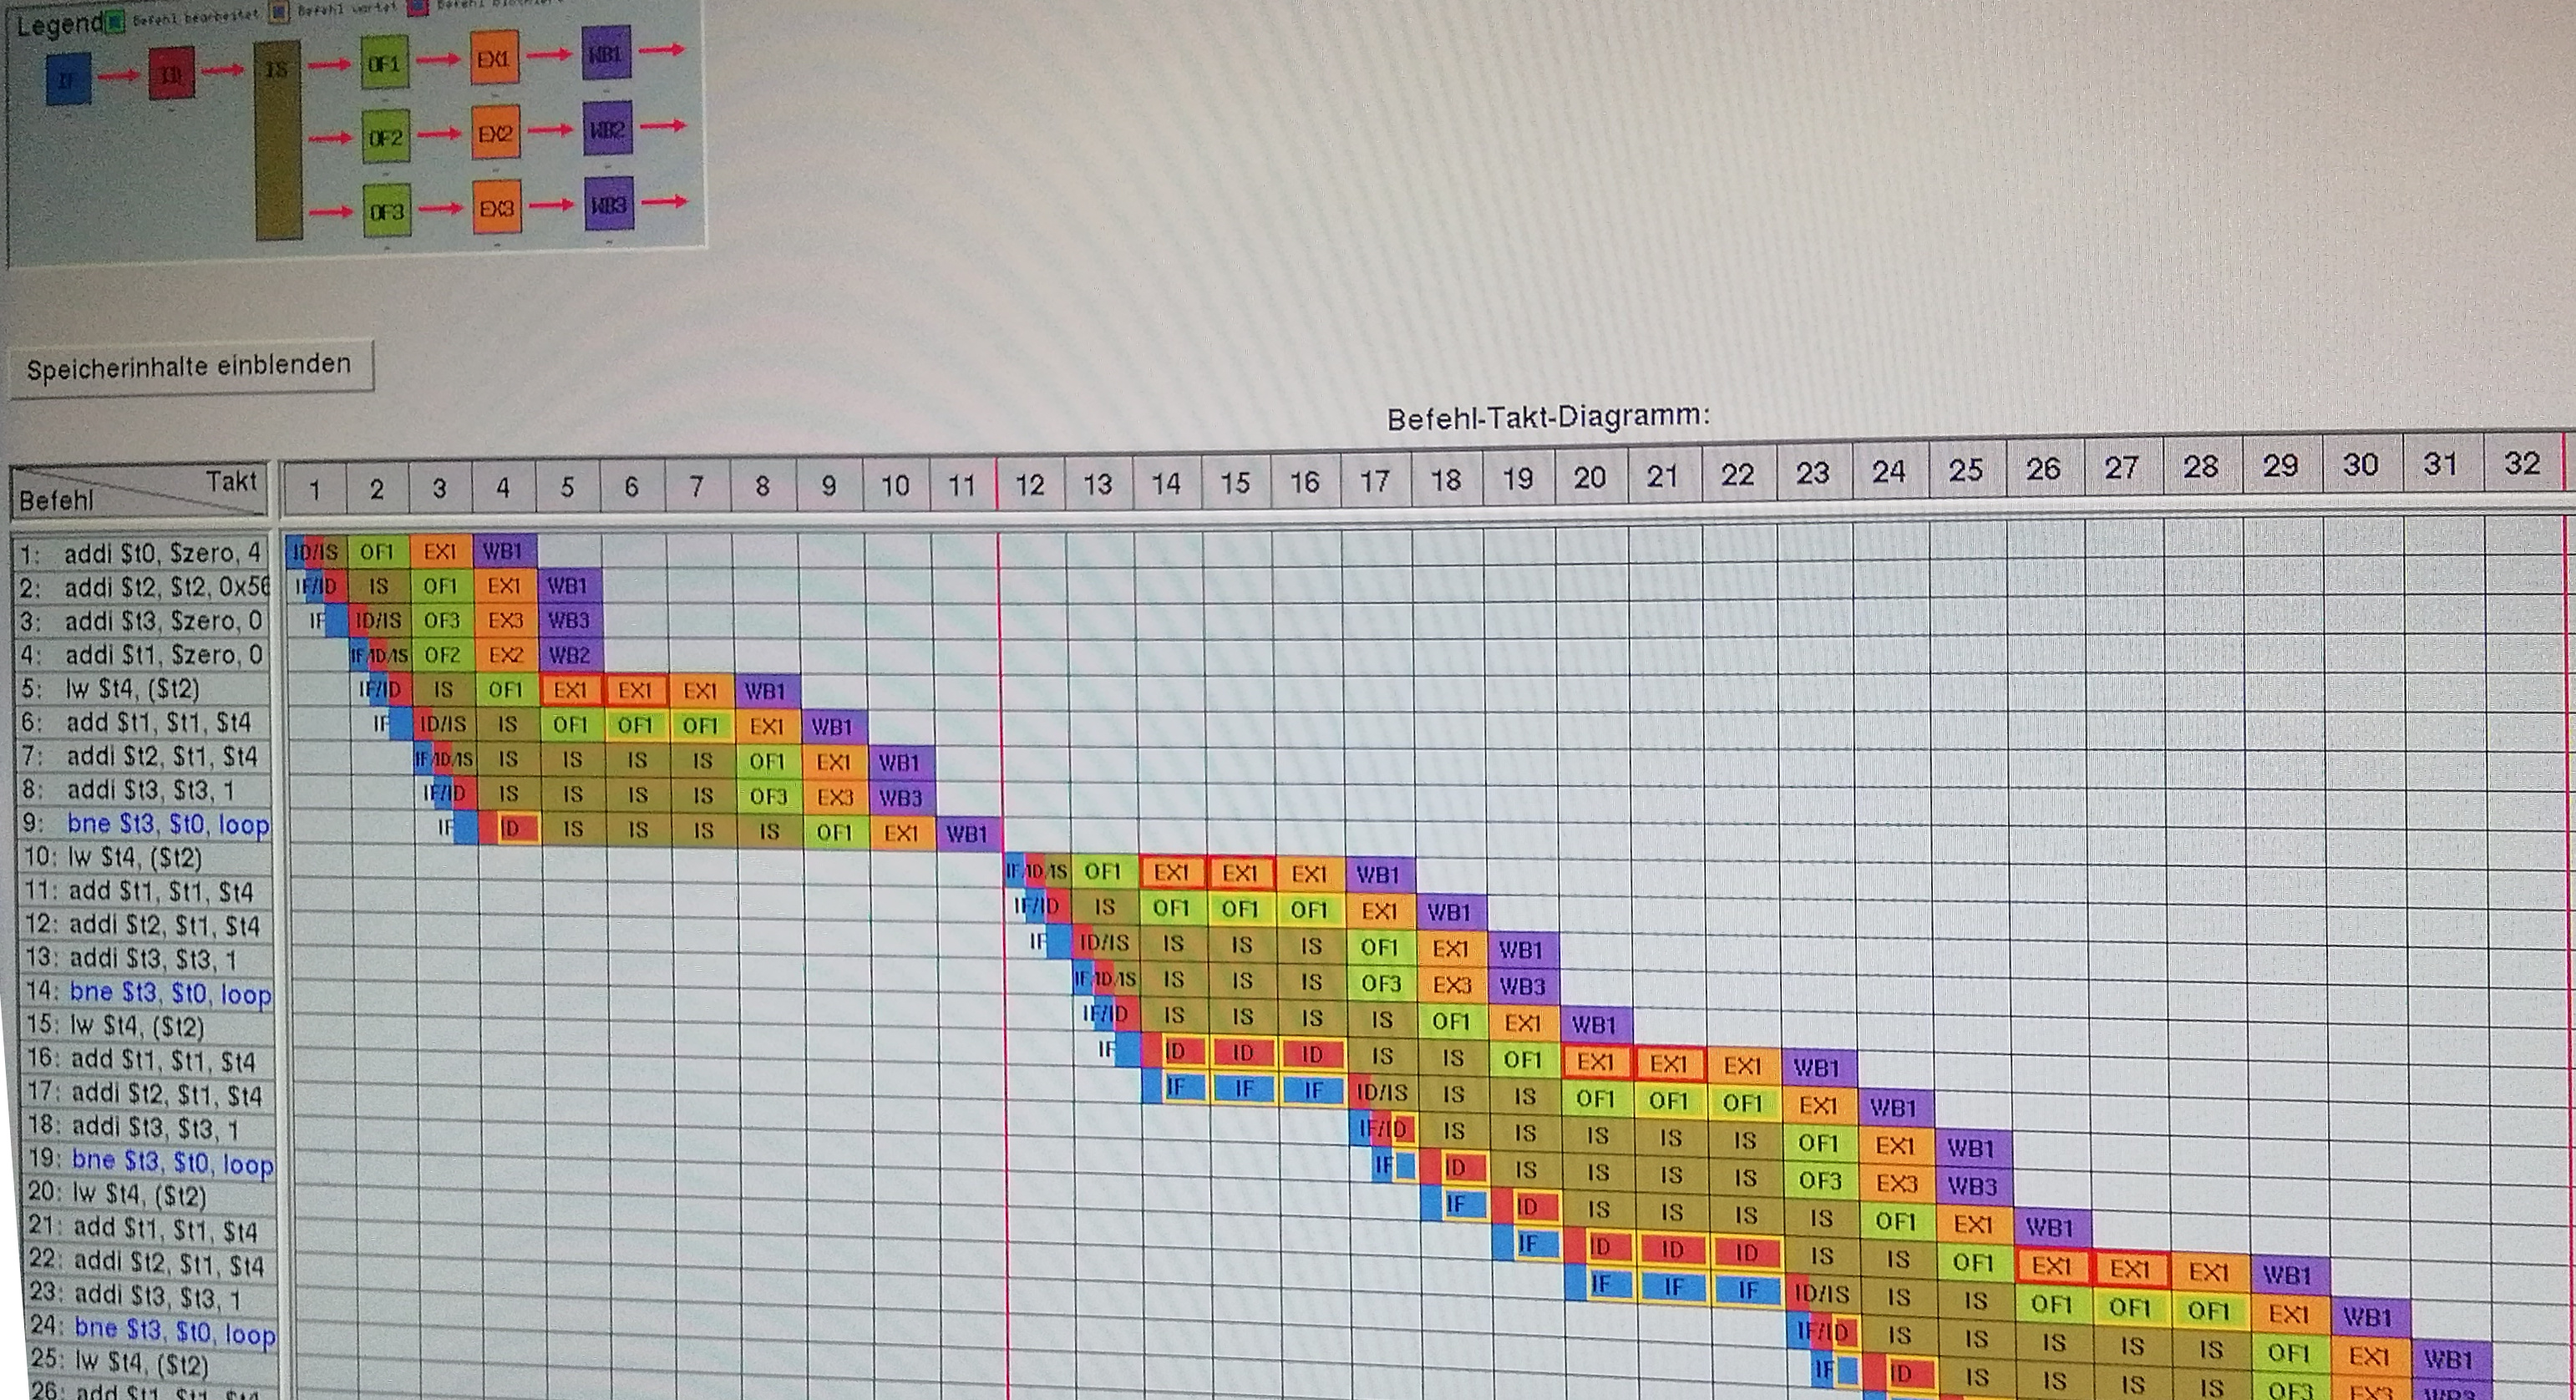
\includegraphics[width=.4\linewidth]{Assets/RA2-65225.jpg}
    \end{itemize*}
    \item Superskalar In-Order Pipeline (2 EX Einheiten)
    \begin{itemize*}
        \item 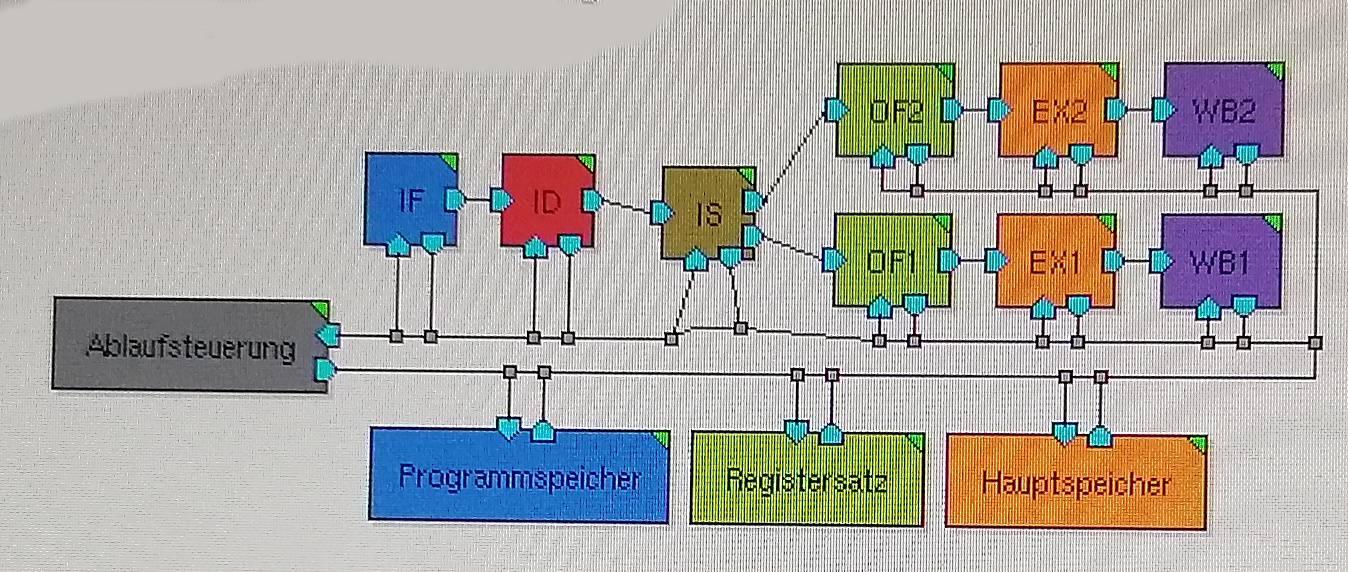
\includegraphics[width=.4\linewidth]{Assets/RA2-65346.jpg}
        \item Takte: 34
        \item Befehle: 30
        \item 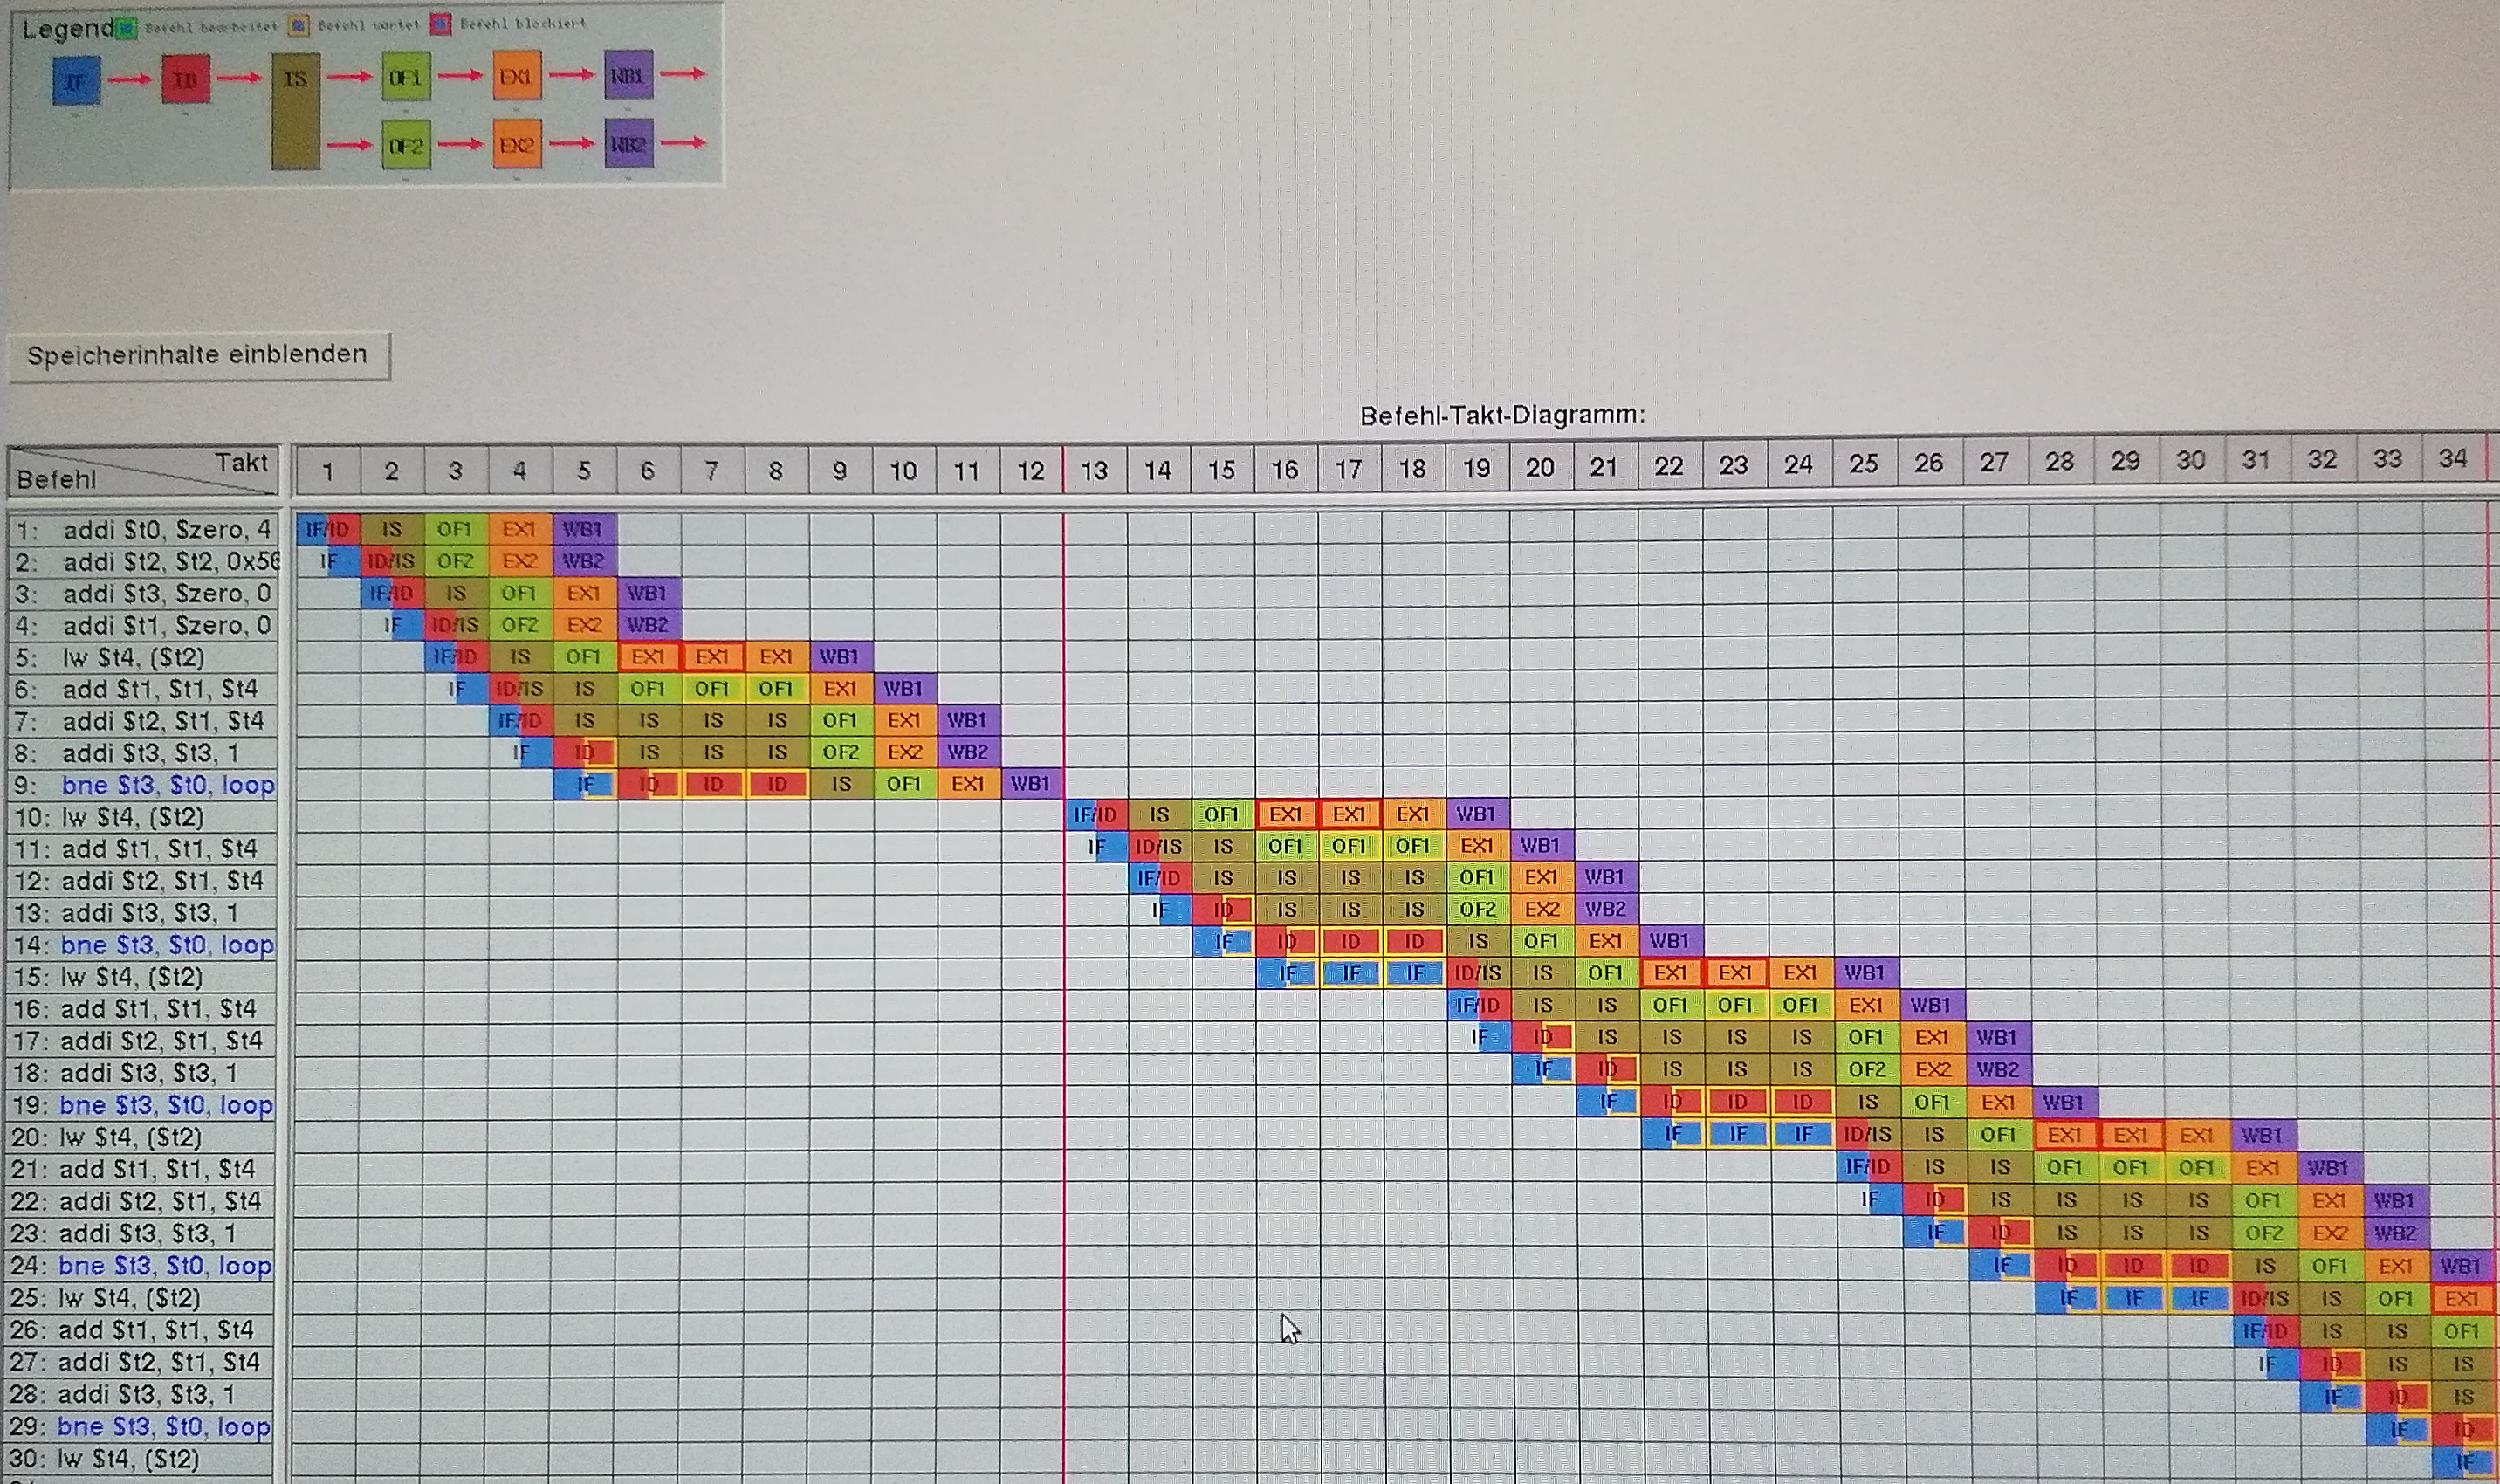
\includegraphics[width=.4\linewidth]{Assets/RA2-65517.jpg}
    \end{itemize*}
    \item Superskalar Out-of-Order ( 3 EX Einheiten)
    \begin{itemize*}
        \item 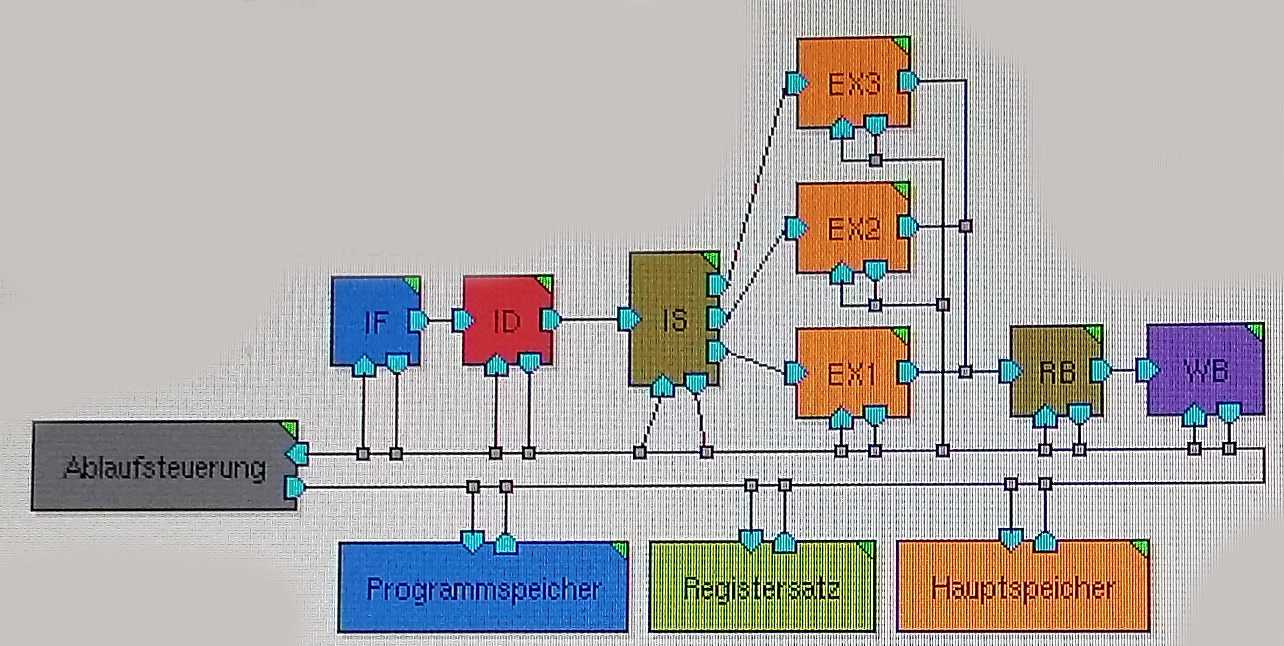
\includegraphics[width=.4\linewidth]{Assets/RA2-65743.jpg}
        \item Takte: 28
        \item Befehle: 62
        \item 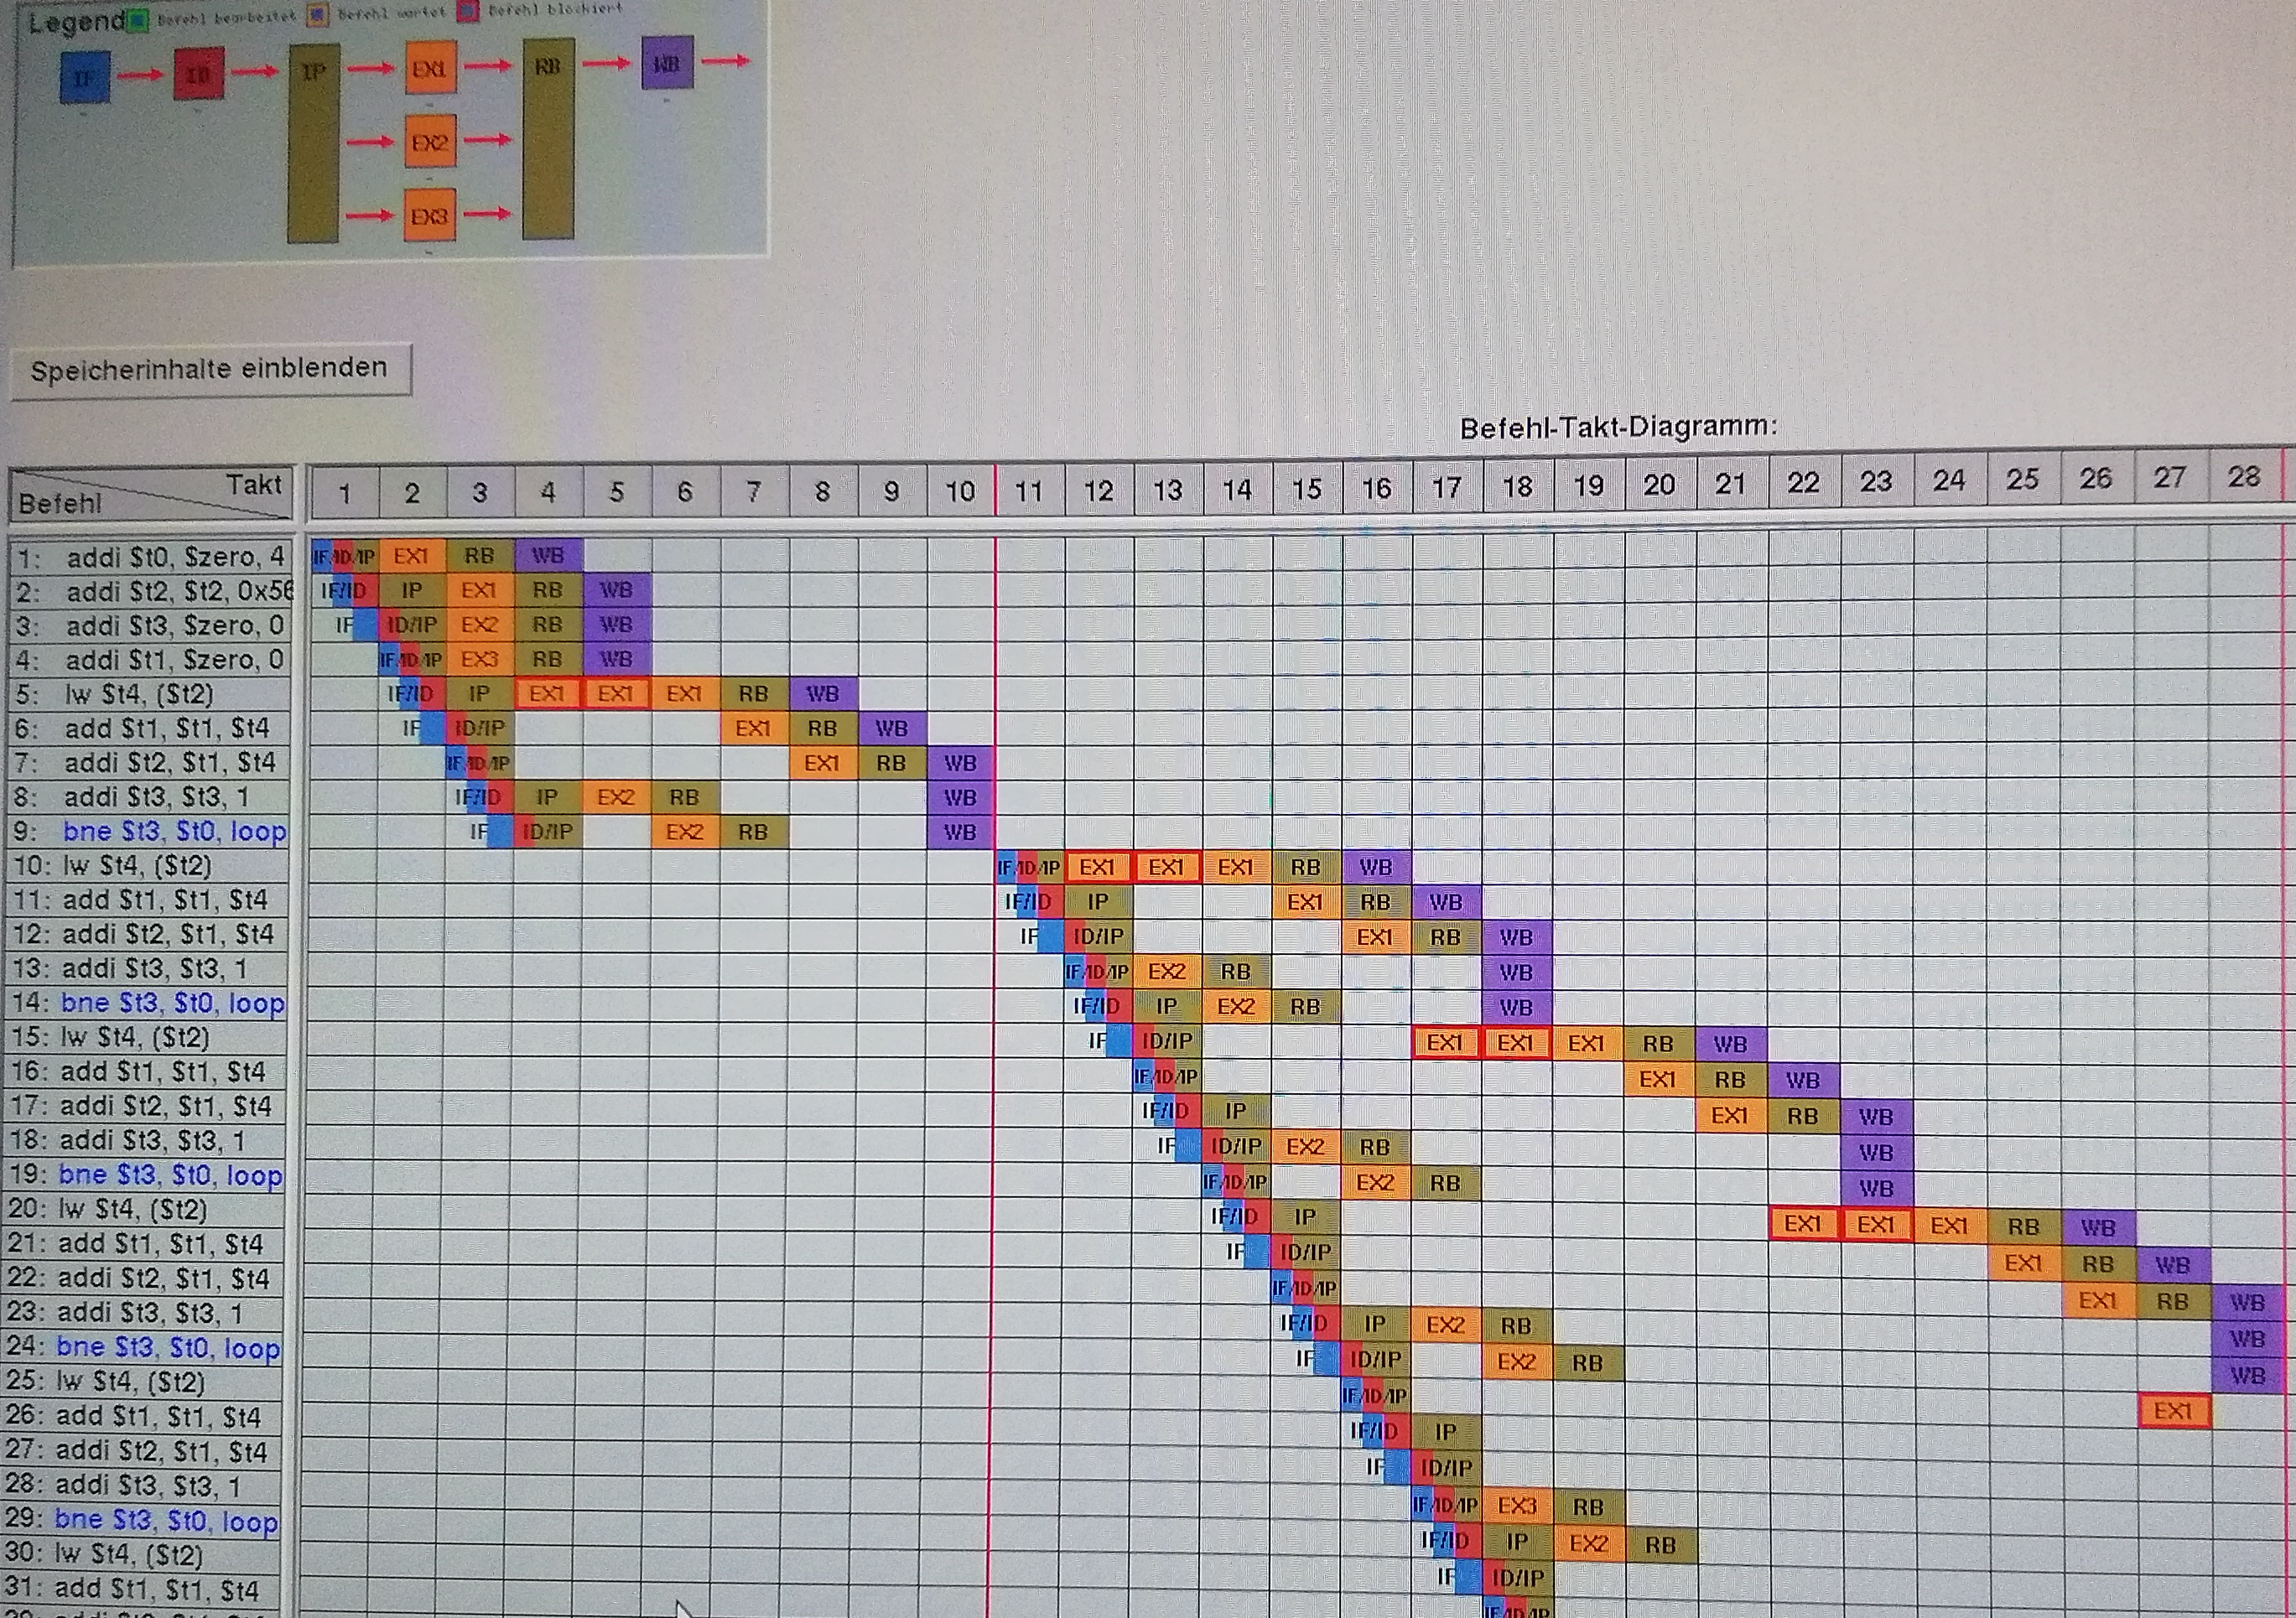
\includegraphics[width=.4\linewidth]{Assets/RA2-70806.jpg}
    \end{itemize*}
    \item Superskalar Out-of-Order ( 2 EX Einheiten)
    \begin{itemize*}
        \item Takte: 30
        \item Befehle: 46
        \item 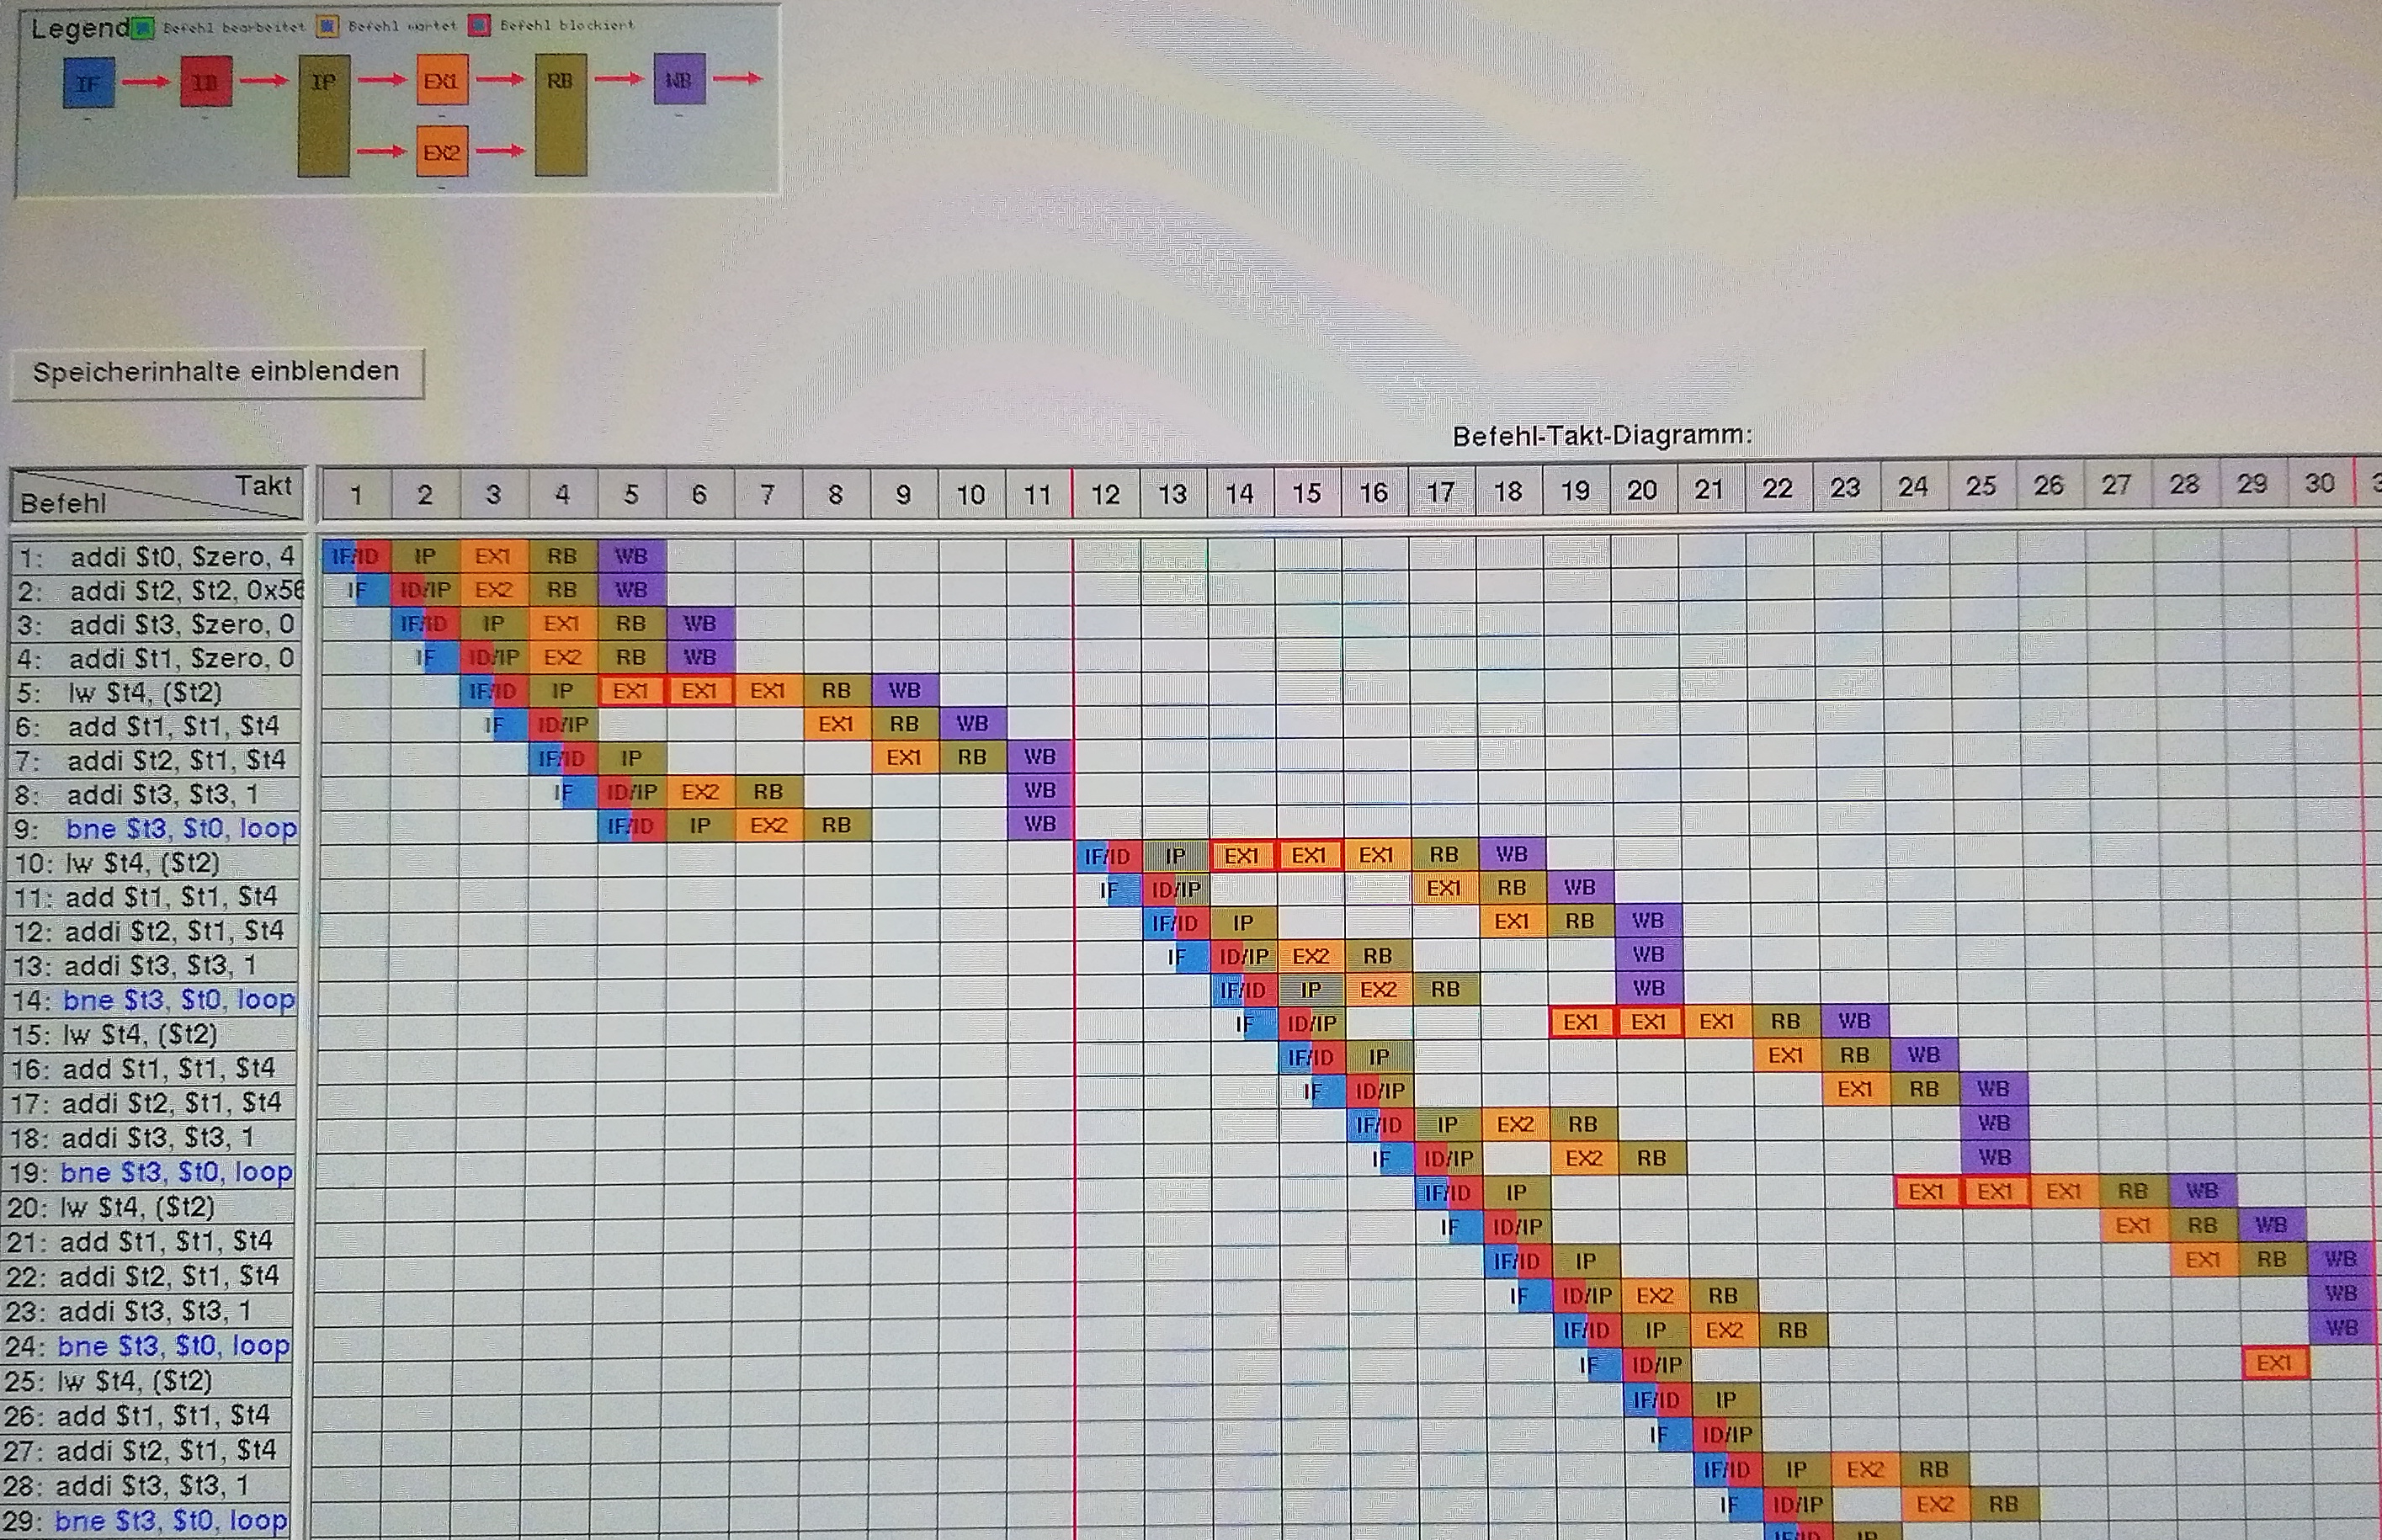
\includegraphics[width=.4\linewidth]{Assets/RA2-70953.jpg}
    \end{itemize*}
    \item Superskalar Out-of-Order ( 9 EX Einheiten)
    \begin{itemize*}
        \item Takte: 27
        \item Befehle: 165
    \end{itemize*}
\end{itemize*}

\subsection*{Zusatzaufgaben}
\subsubsection*{Z1}
Untersuche weitere Befehlsfolgen, z.B. aus A5, A6, A7, B1 oder nach eigenen Entwürfen!

Code A5
\begin{lstlisting}[basicstyle=\tiny]
    addiu   $t1, $zero, 3       #$t1:=3
    addiu   $t2, $zero, 0       #$t2:=0
loop: addu  $t2, $t2, $t1       #$t2:=$t2+$t1
    addiu   $t1, $t1, -1        #$t1:=$t1-1
    bnez    $t1, loop           #branch loop (if $t1<>0)
    or      $t3, $zero, $t1     #$t3:=$t1
    sll     $t4, $t1, 2         #$t4:=$t1 << 2
    and     $t5, $t1, $t5       #$t5:=$t5 AND $t1
    or      $t6, $t1, $t6       #$t6:=$t6 OR $t1
\end{lstlisting}

Code A6
\begin{lstlisting}[basicstyle=\tiny]
        addiu   $t1, $zero, 100
loop1:  addiu   $t2, $zero, 100
loop2:  addiu   $t2, $t2, -1
        ...
        ...
        bnez    $t2, loop2
        addiu   $t1, $t1, -1
        bne     $t1, 1, loop1
\end{lstlisting}

Code A7
\begin{lstlisting}[basicstyle=\tiny]
        addiu   $t1, $zero, 991
loop:   ...
        addu    $t2, $zero, $t1
        and     $t2, $t2, 0x08
        bnez $t2, next
        ...
next:   ...
        addiu $t1, $t1, -1
        bne
        $t1, -1, loop
\end{lstlisting}

Code B1
\begin{lstlisting}[basicstyle=\tiny]
add     $t5, $zero, $t2
add     $t4, $t6, $t5
add     $t3, $t7, $t3
lw      $t0, ($t3)
add     $t7, $zero, $t2
add     $t1, $t6, $t0
sw      $t5, ($t1)
sub     $t2, $t5, $t6
addi    $t4, $zero, 0
addi    $t3, $t3, 1
\end{lstlisting}

\subsubsection*{Z2}
Nehme weitere Änderungen an Parametern und Pipelinestrukturen vor!

\subsubsection*{Z3}
Versuche Befehlsfolgen zu finden, die die strukturellen Ressourcen besonders gut ausnutzen oder die Wirksamkeit bestimmter Methoden (wie z.B. Sprungvorhersagen) besonders gut sichtbar werden lassen!

\newpage
\section*{Versuch M: Mikrocontroller}
Assemblerprogrammierung mit dem 8-Bit-Mikrocontroller ATtiny25

\subsection*{Aufgabe 1: Ein- und Ausschalten der LED}
In dieser Teilaufgabe soll die LED über die beiden Taster ein-, aus- und umgeschaltet werden. Dazu
ist eine funktionierende Teillösung vorgegeben, welche Sie anschließend erweitern sollen.

\subsubsection*{Schritt a: Start der Entwicklungsumgebung}
Geben Sie das folgende Programm ein. Es soll die vorhandenen Befehle ersetzen.
\begin{lstlisting}[basicstyle=\tiny]
.INCLUDE "tn25def.inc"      // Einfügen von Symbolen, u.a. für I/O-Register
.DEVICE ATtiny25            // Festlegen des Controllertyps
anf:
    ldir    16,0x07
    out     DDRB,r16        // Port B: Richtungseinstellung
    ldi     r16,0x18
    out     PORTB,r16       // Port B: Pull-up für Taster-Eingänge aktivieren
lo1:
    sbis    PINB,PB4        // Abfrage TASTER1, Skip Folgebefehl wenn nicht gedrückt
    sbi     PORTB,0         // Einschalten der LED (blau)
    sbis    PINB,PB3        // Abfrage TASTER2, Skip Folgebefehl wenn nicht gedrückt
    cbi     PORTB,0         // Ausschalten der LED (blau)
    rjmp    lo1             // Sprung zum Schleifenbeginn
\end{lstlisting}

\subsubsection*{Schritt b: Manuelle Farbwechsel der LED}
Das Programm soll jetzt so erweitert werden, dass die LED mit den beiden Tastern zwischen zwei Leuchtfarben umgeschaltet werden kann.
\begin{lstlisting}[basicstyle=\tiny]
\end{lstlisting}

Verändern Sie das Programm nun so, dass durch abwechselndes Drücken der beiden Taster eine Sequenz von mindestens sechs unterschiedlichen Leuchtvarianten der LED durchgeschaltet werden kann.
\begin{lstlisting}[basicstyle=\tiny]
\end{lstlisting}

\subsection*{Aufgabe 2: Blinken der LED}
In dieser Teilaufgabe soll das Programm die LED fortlaufend blinken lassen. Diese Funktion wird mit einem Zähler/Zeitgeber-Interrupt realisiert.

\subsubsection*{Schritt a: Einfaches Blinken}
Die Aufgabe besteht nun darin, die LED periodisch ein- und auszuschalten, so dass sich eine Frequenz von etwa 2 Hz ergibt. Das Umschalten der LED soll in der Interruptserviceroutine eines Zähler/Zeitgeber-Interrupts erfolgen. Dafür soll Timer/Counter 0 so initialisiert werden, dass er Interrupts mit einer Folgefrequenz von etwa 4 Hz auslöst.

Stützen Sie sich dazu auf das folgende Programmfragment:
\begin{lstlisting}[basicstyle=\tiny]
// Interrupttabelle (muss vor dem ersten ausführbaren Befehl stehen):
tab: rjmp   anf // Programmstart nach Reset ("Interrupt" 1)
    reti
    reti
    reti
    reti
    reti
    reti
    reti
    reti
    reti
    rjmp    i_11 // Timer 0 Compare A Interrupt (Interrupt 11)
    reti
    reti
    reti
    reti    // Tabellenende (Interrupt 15)

// Initialisierungsteil und Hintergrundprogramm:
anf: [...]  // Weitere Initialisierungen
     [...]  // Initialisierung von Timer/Counter 0 (Empfehlung:
            // Betriebsart CTC, Vergleichsregister A nutzen)
    sei     // Globale Interruptfreigabe
    ldi r16,0x10
    out TIMSK,r16   // Freigabe von Interrupt 11 (Timer 0 Compare A)
lo2: rjmp   lo2     // Leere Hintergrundschleife

// Interruptserviceroutine:
i_11: in    r25,SREG    // Flags retten (weitere Rettungen nach Bedarf)
    [...]               // Inhalt der Routine
    out     SREG,r25    // Flags restaurieren
    reti                // Routine beenden
\end{lstlisting}

Die Hintergrundschleife bleibt zunächst leer. Entwickeln und testen Sie das Programm für diese Aufgabe.

\subsubsection*{Schritt b: Erweitertes Blinken}
Bauen Sie in die Hintergrundschleife eine Abfrage von TASTER1 und TASTER2 ein. Durch Drücken von TASTER1 soll die Blinkfrequenz verdreifacht werden, durch TASTER2 wird sie auf den ursprünglichen Wert zurückgestellt.
Testen Sie diese Funktion. Der Vorgang soll sich beliebig wiederholen lassen.
Stellen Sie das Programm nun so um, dass die beiden Blinkfrequenzen deutlich langsamer sind: Etwa 1,0 Hz und etwa 0,5 Hz. Beachten Sie, dass der Zählumfang des Timer/Counter dafür nicht ausreicht, auch nicht mit dem größten Vorteiler. Sie müssen das Programm also in der Struktur verändern.
Erweitern Sie das Programm so, dass eine Sequenz aus mindestens vier unterschiedlichen Leuchtzuständen durchlaufen wird. Sie können dabei nach Belieben auch komplexere Abläufe realisieren.

Optional: Stellen Sie die Tasterabfrage auf Interruptbetrieb um. Hierfür bietet sich der ,,Pin Change Interrupt'' an. Beachten Sie, dass wegen des Prellens der Taster ein einzelner Tastendruck eine ganze Serie von Interrupts auslösen kann.

Optional: Realisieren Sie eine Entprellung der Taster. Dazu ist nach jeder erkannten Änderung des Zustands eines Tasters eine Wartezeit von z.B. 0,2 s nötig, während derer weitere Zustandswechsel dieses Tasters ignoriert werden. Auf der Grundlage entprellter Taster können Sie erweiterte Umschaltfunktionen implementieren, bei denen auch das mehrmalige Drücken desselben Tasters eine Rolle spielt.

\subsection*{Aufgabe 3: Einfaches Dimmen der LED mittels PWM}
In dieser Aufgabe soll die Helligkeit der LED mittels PWM (pulse width modulation, Pulsbreitenmodulation) auf wählbare Zwischenwerte eingestellt werden.

\subsubsection*{Schritt a: Einfache Helligkeitseinstellung}
Zunächst soll die LED (nur eine Farbe) auf eine beliebige, aber konstante Helligkeit eingestellt werden können. Realisieren Sie dazu eine PWM-Ausgabe mit 256 Helligkeitsstufen, wobei Sie die Zeitintervalle wahlweise mittels Zählschleifen oder mittels Timer/Counter-Interrupt generieren. Den Helligkeitswert können Sie über ein Universalregister vorgeben, in welches Sie im Debugger bei gestopptem Programm jeweils unterschiedliche Werte eintragen.
Alternativ können Sie auch die PWM-Betriebsarten der Timer/Counter-Baugruppen ausprobieren, soweit es die Hardwarekonfiguration zulässt. Empfohlen wird die Betriebsart ,,Fast PWM'' mit normaler Zählung.

\subsubsection*{Schritt b: Helligkeitseinstellung mit Tastern}
Nun sollen die beiden Taster als Bedienelemente zum Auf- und Abdimmen verwendet werden. Werten Sie dabei die Dauer der Tastendrücke aus, nicht deren Anzahl. Die Helligkeit soll bei gedrückt gehaltenem Taster stetig zu- oder abnehmen. Bei losgelassenen Tastern soll die Helligkeit konstant bleiben.

\subsection*{Zusatzaufgabe: Fortlaufendes Auf- und Abdimmen der LEDs}
Diese Aufgabe soll als Anregung für weiterführende Experimente nach eigenen Ideen dienen. In Absprache mit dem Betreuer können Sie andere Aufgabenteile weglassen, falls Sie die Zusatzaufgabe unter Einbeziehung umfangreicher eigener Ideen in Angriff nehmen wollen.

Die Helligkeit der LED soll in einer geeigneten Geschwindigkeit stetig herauf- und heruntergeregelt werden, so dass ein ,,weiches Blinken'' entsteht. Dazu müssen Sie einen Mechanismus implementieren, der den Helligkeitswert nach einem geeigneten Zeitschema verändert.
Realisieren Sie weitere Lichteffekte dieser Art, bei denen nun auch mehrere Leuchtfarben beteiligt sind.
Realisieren Sie eine Umschaltung zwischen unterschiedlichen Lichteffekten.
Realisieren Sie weitergehende Funktionen nach eigenen Ideen.

\end{document}

